\section{Claude Shannon and the Invention of Information Theory (1940)}


\subsection{Shannon and the Birth of Information Entropy}

While Kolmogorov was grounding probability theory in measure theory, a young American mathematician named \textbf{Claude Shannon} was asking a very different question: \emph{how do we measure information?}

It’s easy to forget that before Shannon, there was no rigorous way to describe information. People used the word loosely—like "data" or "knowledge"—but no one could say exactly what it was, much less quantify it. Shannon changed all that with his 1948 paper, \emph{A Mathematical Theory of Communication}, laying the foundations of modern digital communication. In it, he introduced a precise, mathematical way to quantify \emph{information}—and in doing so, he forever changed the landscape of communication, computation, and probability theory.

Shannon’s core insight was that information is fundamentally about \emph{uncertainty}. The more unpredictable a message, the more information it carries when revealed. To quantify this, he borrowed a term from thermodynamics: \textbf{entropy}.

He defined the entropy of a discrete random variable \( X \), with probability distribution \( \{p_i\} \), as:
\[
H(X) = - \sum_i p_i \log_2 p_i
\]

This quantity, now known as \emph{Shannon entropy}, measures the average number of binary (yes/no) questions required to identify an outcome drawn from \( X \). In other words, it captures the minimum number of bits needed to encode the message without loss.





According to Shannon himself, he wasn’t initially sure what to call this new quantity. He asked mathematician \textbf{John von Neumann} for advice, and von Neumann replied:

\begin{quote}
“Call it entropy. No one knows what entropy really is, so in a debate, you will always have the advantage.”
\end{quote}

The name stuck—but it was more than a clever rhetorical move. Shannon’s entropy wasn’t just metaphorically related to thermodynamic entropy; it was mathematically analogous. 

To understand just how deep this analogy runs, and how we arrived at a point where heat, probability, and information all share the same mathematical structure, we need to go back. Before Shannon, before even Boltzmann, there was a puzzle about steam engines—and the story begins with Sadi Carnot.


\subsection{An Example of Entropy: The Case of the Hidden Marble}

To see what Shannon meant by entropy, let’s start with a simple puzzle.

Suppose you have a bag with \textbf{8 marbles}, and exactly one of them is painted red on the inside. You don’t know which one, and you’re not allowed to peek inside the bag. Instead, you’re allowed to ask a series of yes/no questions to figure out which marble is red.

How many questions will it take?

If your questions are clever—like “Is the red marble in the first half of the bag?”—you can eliminate half the possibilities with each answer. After one question, you’re down to 4 marbles. After two, 2 marbles. After three questions, you know exactly which marble is red.

\[
\log_2(8) = 3
\]

So the entropy of this system—the number of bits of information needed to resolve the uncertainty—is \textbf{3 bits}. This is what Shannon entropy measures: how many yes/no decisions you’d need, on average, to identify the true state of a system.

\medskip

Now imagine you had 16 marbles. You’d need 4 bits.

With 128 marbles? That’s:

\[
\log_2(128) = 7
\]

So finding the special marble takes 7 yes/no questions. The more possibilities there are, the higher the uncertainty—and the more information you need to resolve it. That’s entropy.

\medskip

In essence: \textit{Entropy is how many questions you need to stop guessing.}


\begin{tcolorbox}[title={\textbf{Historical Sidebar: Spencer-Brown and the Primordial Bit}}, colback=gray!5, colframe=black, fonttitle=\bfseries]

  In his 1969 work \emph{Laws of Form}, polymath \textbf{George Spencer-Brown} offered a strikingly minimalist foundation for logic and mathematics. He argued that the most fundamental operation of thought is not computation or deduction, but something even simpler: \textbf{making a distinction}.

  \medskip
  
  To distinguish is to carve the world into parts. Draw a line on a blank surface and you have defined an \emph{inside} and an \emph{outside}—a primitive yes/no, a 1 and 0. In this way, the act of distinction is the ur-form of information: it creates the space in which bits can exist.
  
  \medskip
  
  This idea echoes Shannon’s concept of entropy. When Shannon defines information as the number of yes/no questions needed to resolve uncertainty, he is effectively \textbf{counting the distinctions} required to identify a hidden state. Each question divides the space of possibilities—just like Spencer-Brown’s mark on a page.
  
  \medskip
  
  But Spencer-Brown goes further: he notes that even the blank page—our supposed starting point—is already a distinction. The very notion of a “formless background” only exists because we have already distinguished it from something else. In this sense, distinction is not only the beginning of logic but the precondition for \textbf{any system}.
  
  \begin{quote}
    A universe comes into being when a space is severed or taken apart. The skin of a living organism cuts off an outside from an inside. So does the circumference of a circle in a plane.  --- \textit{Laws of Form}
  \end{quote}
  
\end{tcolorbox}


\subsection{The Origins of Entropy: From Waterwheels to Heat Engines}

Before entropy became a pillar of modern physics, it was born out of a puzzle: why are steam engines less efficient than waterwheels?

In the early 19th century, French engineer \textbf{Sadi Carnot} sought to answer this question. At the time, the dominant understanding of heat was the \emph{caloric theory}, largely shaped by chemist \textbf{Antoine Lavoisier}. According to this theory, heat—called \emph{caloric}—was considered a weightless, invisible fluid that could flow but not be created or destroyed. It acted like a conserved substance that moved from hot bodies to cold ones, much like water flowing downhill.

Carnot leaned into this idea and asked: if caloric is like a fluid, could a steam engine be understood the same way as a waterwheel?

To explore this, Carnot made a formal analogy between \emph{gravitational potential energy} and \emph{thermal energy}:

\begin{itemize}
  \item In a waterwheel, work is extracted by allowing water to fall from a higher elevation to a lower one.
  \item In a heat engine, Carnot imagined that caloric fell from a higher temperature to a lower one, doing work along the way.
\end{itemize}

Mathematically, the work done by a waterwheel is given by:
\[
W = mg \Delta h
\]
where:
\begin{itemize}
  \item \( m \) is the mass of the water,
  \item \( g \) is the gravitational acceleration,
  \item \( \Delta h \) is the height difference.
\end{itemize}



\begin{figure}[H]
\centering
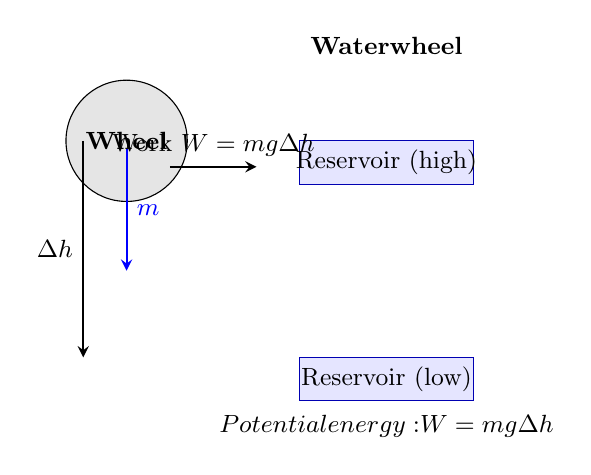
\begin{tikzpicture}[scale=1.1, every node/.style={font=\small}, >=stealth]

% Waterwheel label
\node at (-4,3.1) {\textbf{Waterwheel}};

% Upper reservoir (water)
\draw[fill=blue!10, draw=blue!70!black] (-5,2) rectangle (-3,1.5);
\node at (-4,1.75) {Reservoir (high)};

% Wheel (moved further left)
\draw[fill=gray!20] (-7,2) circle (0.7);
\node at (-7,2) {\textbf{Wheel}};

% Water flow
\draw[->, thick, blue] (-7,1.9) -- (-7,0.5) node[midway, right] {\(m\)};
\draw[->, thick] (-6.5,1.7) -- (-5.5,1.7) node[midway, above] {Work \(W = mg\Delta h\)};

% Lower reservoir
\draw[fill=blue!10, draw=blue!70!black] (-5,-0.5) rectangle (-3,-1);
\node at (-4,-0.75) {Reservoir (low)};

% Height arrow
\draw[->, thick] (-7.5,2) -- (-7.5,-0.5) node[midway, left] {\(\Delta h\)};

% Potential energy formula
\node at (-4,-1.3) {\( \text{Potential energy: } W = mg\Delta h \)};

\end{tikzpicture}
\caption{
A waterwheel extracts work by allowing water of mass \( m \) to fall from a higher reservoir to a lower one through a height difference \( \Delta h \). The gravitational potential energy is converted into mechanical work via the wheel. This classical setup was used by Carnot as a physical analogy to understand how heat engines operate—by converting a falling substance (water or caloric) into useful work.
}
\end{figure}





In Carnot’s analogy:
\begin{itemize}
  \item Temperature \( T \) replaces height \( h \),
  \item Caloric (later recognized as entropy, \( S \)) replaces mass \( m \),
  \item The product \( S \Delta T \) becomes analogous to the mechanical work potential.
\end{itemize}

Thus, the heat transferred in a process becomes:
\[
Q = S \Delta T
\]
where:
\begin{itemize}
  \item \( Q \) is the heat energy carried by caloric,
  \item \( \Delta T \) is the temperature drop,
  \item \( S \) is the amount of caloric (a conserved quantity in this theory).
\end{itemize}




\begin{figure}[H]
\centering
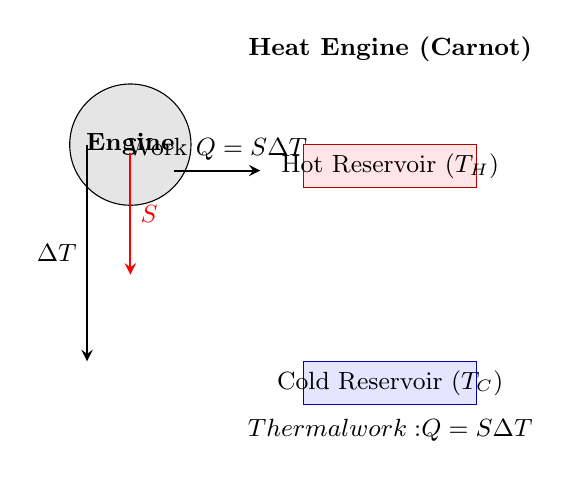
\begin{tikzpicture}[scale=1.1, every node/.style={font=\small}, >=stealth]

% Heat engine label
\node at (2,3.1) {\textbf{Heat Engine (Carnot)}};

% Hot reservoir
\draw[fill=red!10, draw=red!70!black] (1,2) rectangle (3,1.5);
\node at (2,1.75) {Hot Reservoir (\(T_H\))};

% Engine (aligned with waterwheel horizontally)
\draw[fill=gray!20] (-1,2) circle (0.7);
\node at (-1,2) {\textbf{Engine}};

% Caloric flow
\draw[->, thick, red] (-1,1.9) -- (-1,0.5) node[midway, right] {\(S\)};
\draw[->, thick] (-0.5,1.7) -- (0.5,1.7) node[midway, above] {Work \(Q = S\Delta T\)};

% Cold reservoir
\draw[fill=blue!10, draw=blue!70!black] (1,-0.5) rectangle (3,-1);
\node at (2,-0.75) {Cold Reservoir (\(T_C\))};

% Temperature gradient
\draw[->, thick] (-1.5,2) -- (-1.5,-0.5) node[midway, left] {\(\Delta T\)};

% Thermal work formula
\node at (2,-1.3) {\( \text{Thermal work: } Q = S\Delta T \)};

\end{tikzpicture}
\caption{
Carnot’s heat engine model treats heat (originally called caloric) as a conserved fluid flowing from a hot reservoir at temperature \( T_H \) to a cold one at \( T_C \). The work extracted depends on the amount of entropy \( S \) transferred and the temperature difference \( \Delta T \). This analogy to gravitational systems—where potential is tied to height—is what led to the abstract formulation of entropy as a state variable in thermodynamics.
}
\end{figure}



Crucially, in the caloric model, caloric could not be created or destroyed—it could only be moved. That meant for a heat engine to be efficient, it needed to transfer caloric from a hot reservoir to a cold one while extracting the maximum work possible during that “fall.”

Carnot analyzed an idealized engine cycle, later called the \emph{Carnot cycle}, composed of two isothermal (constant temperature) and two adiabatic (no heat exchange) processes. Under the caloric theory, the total caloric input and output must be equal, since caloric is conserved. The efficiency of the engine was then determined purely by the temperatures of the hot and cold reservoirs:
\[
\eta = 1 - \frac{T_C}{T_H}
\]
where \( T_H \) and \( T_C \) are the temperatures of the hot and cold reservoirs, respectively.

This was a profound insight: \emph{no engine could be more efficient than a Carnot engine operating between the same two temperatures}, regardless of its construction.










Although the caloric theory would later be disproven—supplanted by the kinetic theory of heat and the first law of thermodynamics—Carnot’s reasoning turned out to be remarkably accurate. The idea that heat transfer and temperature difference together determine extractable work laid the groundwork for the modern concept of entropy.

Carnot’s work showed that even under a flawed physical model, the right mathematical structure could yield truths that transcend their origins. Entropy, as a quantity that flows and drives work when crossing a temperature gradient, began as a metaphor—but evolved into one of the most powerful ideas in all of science.




\begin{tcolorbox}[colback=gray!5!white, colframe=black!75!white, title={Historical Sidebar: Feyerabend, Caloric, and the Accidental Truth of Error}]

  \textbf{Paul Feyerabend} (1924–1994) was one of the most controversial philosophers of science in the 20th century. Best known for his book \textit{Against Method}, Feyerabend challenged the very idea that science advances through a strict, rational method. He argued instead for \textbf{epistemological anarchism}: the view that “anything goes” when it comes to the history of scientific discovery.
  
  \medskip
  
  One of Feyerabend’s core ideas was \textbf{incommensurability}: the claim that competing scientific theories often operate in different conceptual worlds, making them impossible to directly compare by neutral standards. According to him, the transition from one theory to another (say, from caloric theory to thermodynamics) isn’t always driven by logic and evidence, but by cultural shifts, aesthetic preferences, and even historical accidents.
  
  \medskip
  
  Enter the \textbf{caloric theory}: a theory that posited heat as a conserved fluid called “caloric.” By today’s standards, it’s flat-out wrong. Heat is not a substance; it’s energy in motion. And yet, as Feyerabend might gleefully point out, this flawed theory was crucial in shaping one of the most powerful concepts in physics: \textbf{energy conservation}.
  
  \medskip
  
  Carnot, operating under the caloric framework, developed deep insights about work, heat, and temperature: insights that survived even after the theory itself was abandoned. In fact, it was only by treating heat as a kind of indestructible stuff that Carnot could arrive at the idea of a perfectly efficient engine and lay the groundwork for entropy.
  
  \medskip
  
  \textbf{Feyerabend’s moral?} Science progresses not because it always gets things “right,” but because even wrong ideas can open the door to profound truths. The caloric theory didn’t just fail—it failed \textit{productively}.

  \medskip
  
  \begin{quote}
  \textit{“The only principle that does not inhibit progress is: anything goes.”} —Paul Feyerabend, \textit{Against Method}
  \end{quote}
  
\end{tcolorbox}
  

\subsection{From Heat Engines to Microstates: Boltzmann’s Statistical Revolution}

Imagine a box filled with gas. If all the molecules were somehow trapped in one corner, the system would look remarkably ordered—but also extremely unlikely. Now imagine the molecules bouncing around freely, evenly filling the box. That’s the most natural, “random-looking” state—and also the most probable.

\begin{figure}[H]
\centering
\begin{tikzpicture}[scale=0.55, every node/.style={font=\small}, dot/.style={circle, fill=black, minimum size=4pt, inner sep=0pt}]

% Helper to draw grid
\newcommand{\drawgrid}[2]{
  \begin{scope}[shift={(#1,#2)}]
    \foreach \x in {0,...,5} {
      \foreach \y in {0,...,5} {
        \draw (\x,\y) rectangle +(1,1);
      }
    }
  \end{scope}
}

% === Top-left: All in corner ===
\drawgrid{0}{7}
\foreach \x in {0,1} {
  \foreach \y in {4,5} {
    \node[dot] at (\x + 0.5, \y + 0.5 + 7) {};
  }
}
\node at (3,6.5) {\textbf{\footnotesize All in Corner}};

% === Top-right: Clustered in region ===
\drawgrid{9}{7}
\foreach \x/\y in {0.5/0.5, 1.5/2.5, 2.5/1.5, 2.5/3.5, 1.5/3.5} {
  \node[dot] at ({9+\x}, {7+\y}) {};
}
\node at (12,6.5) {\textbf{\footnotesize Clustered in Region}};

% === Bottom-left: Half spread ===
\drawgrid{0}{0}
\foreach \x/\y in {0.5/0.5, 1.5/2.5, 2.5/1.5, 3.5/4.5, 4.5/3.5, 5.5/0.5} {
  \node[dot] at ({\x}, {\y}) {};
}
\node at (3,-0.5) {\textbf{\footnotesize Half Spread}};

% === Bottom-right: Evenly spread ===
\drawgrid{9}{0}
\foreach \x/\y in {
  0.5/0.5, 1.5/1.5, 2.5/2.5, 3.5/3.5, 4.5/4.5, 5.5/5.5,
  0.5/5.5, 1.5/4.5, 2.5/3.5, 3.5/2.5
} {
  \node[dot] at ({9+\x}, {\y}) {};
}
\node at (12,-0.5) {\textbf{\footnotesize Evenly Spread}};

\end{tikzpicture}
\caption{
Four macrostates of molecules in a 6×6 grid, increasing in disorder from top-left to bottom-right. 
Top-left: all molecules cluster in a corner — a highly specific and improbable configuration. 
Top-right: slightly more spread out, but still relatively constrained. 
Bottom-left: a more distributed arrangement. 
Bottom-right: molecules are evenly spread — a state that can result from many different underlying arrangements and is thus statistically dominant.
}
\end{figure}






This simple thought experiment captures Ludwig Boltzmann’s great insight: the concept of entropy can be explained by counting.

Each way of arranging the molecules—each exact specification of position and velocity for every particle—is called a \textbf{microstate}. But as observers, we usually only care about large-scale features like temperature and pressure. These macroscopic conditions are called \textbf{macrostates}, and crucially, many different microstates can correspond to the same macrostate.

In our gas example:
\begin{itemize}
  \item The macrostate “all molecules evenly spread” corresponds to an enormous number of possible microstates.
  \item The macrostate “all molecules in one corner” corresponds to far fewer microstates.
\end{itemize}

Boltzmann realized that the more microstates correspond to a macrostate, the more likely it is to occur. 






\begin{figure}[H]
\centering
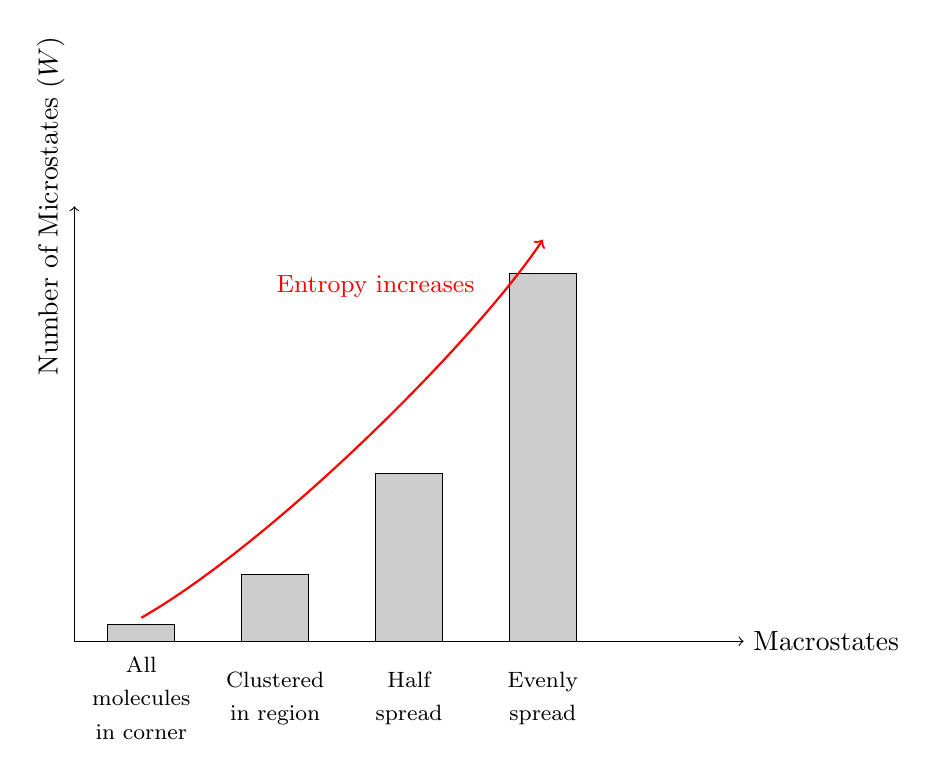
\begin{tikzpicture}[scale=0.85, yscale=0.05]

% Axes
\draw[->] (0,0) -- (10,0) node[right] {Macrostates};
\draw[->] (0,0) -- (0,130) node[above, rotate=90] {Number of Microstates (\( W \))};

% Bars with horizontal spacing
\draw[fill=gray!40] (0.5,0) rectangle (1.5,5);    % All in corner
\draw[fill=gray!40] (2.5,0) rectangle (3.5,20);   % Clustered
\draw[fill=gray!40] (4.5,0) rectangle (5.5,50);   % Half spread
\draw[fill=gray!40] (6.5,0) rectangle (7.5,110);  % Evenly spread

% Labels under bars with further vertical offset
\node[align=center] at (1.0,-17) {\footnotesize All\\\footnotesize molecules\\\footnotesize in corner};
\node[align=center] at (3.0,-17) {\footnotesize Clustered\\\footnotesize in region};
\node[align=center] at (5.0,-17) {\footnotesize Half\\\footnotesize spread};
\node[align=center] at (7.0,-17) {\footnotesize Evenly\\\footnotesize spread};

% Optional: entropy arrow
\draw[->, thick, red] (1.0,7) .. controls (3.0,30) and (6.0,90) .. (7.0,120);
\node[red, above] at (4.5,100) {\small Entropy increases};

\end{tikzpicture}
\caption{
Each macrostate (e.g., “all molecules in one corner” vs. “evenly spread”) corresponds to a different number of compatible microstates \( W \). Boltzmann’s insight was that macrostates with more microstates are overwhelmingly more probable. His formula \( S = k \log W \) shows that entropy increases as the count of indistinguishable configurations grows. This bar chart illustrates how disordered macrostates dominate, not by preference, but by combinatorics.
}
\end{figure}






And he went further—he quantified this intuition.

He proposed that the \textbf{entropy} \( S \) of a system is related to the number of compatible microstates \( W \) via the formula:
\[
S = k \log W
\]
where:
\begin{itemize}
  \item \( S \) is the entropy,
  \item \( k \) is Boltzmann’s constant,
  \item \( W \) is the number of microstates that realize the macrostate.
\end{itemize}

To see how \( W \) can be computed, imagine a simple system: distributing \( N \) indistinguishable molecules into \( M \) distinguishable boxes. Each possible arrangement (microstate) depends on which boxes the molecules land in.

For instance, consider 10 molecules and 2 boxes. The number of ways we can have exactly \( n \) molecules in Box 1 and \( N - n \) in Box 2 is given by the binomial coefficient:
\[
W(n) = \binom{10}{n}
\]
The macrostate is defined by how many molecules are in each box. For example, "5 in Box 1 and 5 in Box 2" is one macrostate. But there are:
\[
W(5) = \binom{10}{5} = 252
\]
ways to realize that — i.e., 252 microstates that all look the same macroscopically.

Compare that to the macrostate "all 10 in one box":
\[
W(10) = \binom{10}{10} = 1
\]
Only one way — a highly specific, low-entropy state.

Now apply Boltzmann’s formula:
\[
S = k \log W(n)
\]
You can immediately see how a modest increase in \( W \) produces a much more reasonable increase in entropy when you take the logarithm. This is why entropy increases with disorder: there are simply far more ways to be disordered than ordered.


\begin{figure}[H]
\centering
\begin{tikzpicture}[scale=0.95, every node/.style={font=\small}]

% Axes
\draw[->] (0,0) -- (10.5,0) node[right] {\( n \) molecules in Box 1};
\draw[->] (0,0) -- (0,6) node[above, rotate=90] {\( S = k \log W(n) \)};

% Dots and vertical dashed lines
\foreach \n/\w in {
  0/1,
  1/10,
  2/45,
  3/120,
  4/210,
  5/252,
  6/210,
  7/120,
  8/45,
  9/10,
  10/1
} {
  \pgfmathsetmacro{\x}{\n}
  \pgfmathsetmacro{\y}{ln(\w)}
  \filldraw[blue] (\x, \y) circle (2pt);
  \draw[dashed, gray] (\x,0) -- (\x, \y);
}

% Smooth curve using precomputed coordinates
\draw[smooth, thick, blue] plot coordinates {
  (0, 0.000)
  (1, 2.303)
  (2, 3.807)
  (3, 4.787)
  (4, 5.347)
  (5, 5.529)
  (6, 5.347)
  (7, 4.787)
  (8, 3.807)
  (9, 2.303)
  (10, 0.000)
};

\node[blue] at (5.2,5.9) {\( S = k \log \binom{10}{n} \)};

\end{tikzpicture}
\caption{
Entropy as a function of how many molecules are in Box 1, for a system of 10 indistinguishable molecules and 2 distinguishable boxes. The number of microstates \( W(n) = \binom{10}{n} \) peaks at \( n = 5 \), corresponding to maximal disorder. The entropy \( S = k \log W(n) \) follows a smooth, symmetric curve peaking at this most probable macrostate.
}
\end{figure}


This simple combinatoric model shows how entropy naturally emerges from counting. The most probable macrostate — equal distribution of particles — is also the one with the highest entropy. The logarithm tames the explosive growth of microstates, making entropy a smooth, additive quantity.

This is the essence of Boltzmann’s insight: entropy measures the number of ways a macrostate can happen. And the laws of probability ensure that high-entropy macrostates dominate — not because they’re preferred, but because they’re overwhelmingly more common.




And most importantly, the laws of probability dictate that systems will overwhelmingly evolve toward macrostates with more microstates. That’s not just a trend—it’s the statistical foundation of the Second Law of Thermodynamics.

In Boltzmann’s view:
\begin{quote}
Entropy increases not because the universe seeks disorder, but because disorder vastly outnumbers order.
\end{quote}

This was a radical reimagining of entropy. No longer just a tool for calculating engine efficiency, entropy became a bridge between the microscopic and macroscopic worlds. Boltzmann’s statistical mechanics laid the groundwork for quantum theory, cosmology, and even modern information science.

It began with a simple question: “What is heat made of?”  
The answer, it turned out, was: \emph{probability}.



\begin{tcolorbox}[colback=gray!5!white, colframe=black!75!white, title={Historical Sidebar: Boltzmann vs. the Universe (and the Universe Won)}]

  \textbf{Ludwig Boltzmann} (1844–1906) was one of the most brilliant minds in physics, but also one of its most tragic. His statistical interpretation of entropy was revolutionary: rather than assuming a mechanical, deterministic universe where every effect followed directly from a cause, Boltzmann embraced \textbf{probability} as fundamental. To him, heat and disorder weren’t mysterious forces: they were just the statistics of trillions of particles bouncing around.
  
  \medskip
  
  But his ideas met stiff resistance. In the late 19th century, the dominant view -- especially in Europe -- was that the universe was strictly \textbf{deterministic}. Influential figures like \textbf{Ernst Mach} and many in the German-speaking scientific community saw Boltzmann’s use of atoms and probability as speculative, even metaphysical. Atoms hadn’t been directly observed yet. Probability, they argued, was a sign of ignorance. It was not a tool for building laws of nature.
  
  \medskip
  
  Boltzmann fought back with equations and lectures. But the pushback was relentless. He found himself isolated, ridiculed, and misunderstood. Enlightenment thinkers demanded a deterministic universe and introducing uncertainty as fundamental to the laws of nature was nothing less than heracy.
  
  \medskip
  
  \textbf{The stress broke him.} Boltzmann suffered from severe bouts of depression throughout his life. He believed in a probabilistic world full of chaos; he lived in a professional world that believed in certainties. That contradiction haunted him. Despite growing acceptance of atomic theory near the end of his life, the psychological damage had already taken its toll.
  
  \medskip
  
  In 1906, while vacationing in Italy, Boltzmann took his own life. He died not knowing that, just a few years later, Einstein would vindicate the atomic theory, and quantum mechanics would place probability at the center of physics.
  
\end{tcolorbox}



\subsection{From Microstates to Messages: The Information-Theoretic View of Entropy}

Imagine you’re playing a game: someone is thinking of a letter, and you have to guess which one. If it’s from a random jumble of all 26 letters, you might need up to 5 binary (yes/no) questions to find it—like a high-stakes game of 20 Questions. But if you know the letter is likely to be a vowel, or even more likely to be an "e," your odds improve dramatically. The more predictable the message, the fewer questions you need.




\begin{figure}[H]
\centering
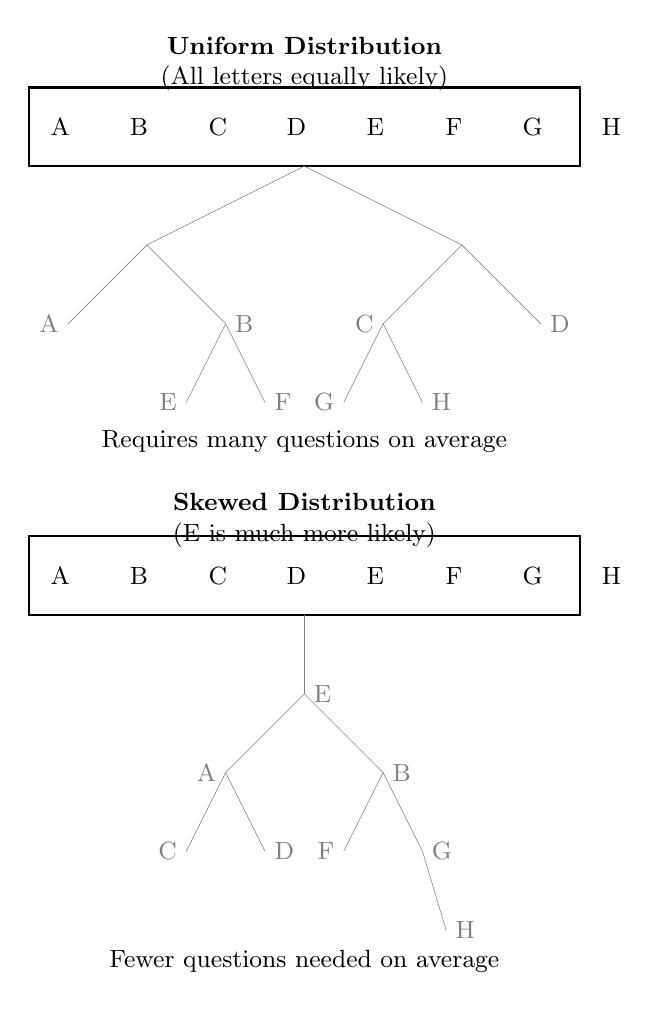
\begin{tikzpicture}[scale=1.0, every node/.style={font=\small}]

% --- Uniform Distribution (Top Panel) ---
\node[align=center] at (0,7.8) {\textbf{Uniform Distribution} \\ (All letters equally likely)};
\draw[thick] (-3.5,6.5) rectangle (3.5,7.5); % box around letters

\foreach \i/\letter in {0/A, 1/B, 2/C, 3/D, 4/E, 5/F, 6/G, 7/H} {
    \node at (-3.1 + \i, 7) {\letter};
}

% Tree for uniform case (balanced)
\draw[very thin, gray] (0,6.5) -- (-2,5.5);
\draw[very thin, gray] (0,6.5) -- (2,5.5);

\draw[very thin, gray] (-2,5.5) -- (-3,4.5) node[left] {A};
\draw[very thin, gray] (-2,5.5) -- (-1,4.5) node[right] {B};
\draw[very thin, gray] (2,5.5) -- (1,4.5) node[left] {C};
\draw[very thin, gray] (2,5.5) -- (3,4.5) node[right] {D};

\draw[very thin, gray] (-1,4.5) -- (-1.5,3.5) node[left] {E};
\draw[very thin, gray] (-1,4.5) -- (-0.5,3.5) node[right] {F};
\draw[very thin, gray] (1,4.5) -- (0.5,3.5) node[left] {G};
\draw[very thin, gray] (1,4.5) -- (1.5,3.5) node[right] {H};

\node at (0,3) {\small Requires many questions on average};

% --- Skewed Distribution (Bottom Panel) ---
\node[align=center] at (0,2.0) {\textbf{Skewed Distribution} \\ (E is much more likely)};
\draw[thick] (-3.5,0.8) rectangle (3.5,1.8); % box around letters

\foreach \i/\letter in {0/A, 1/B, 2/C, 3/D, 4/E, 5/F, 6/G, 7/H} {
    \node at (-3.1 + \i, 1.3) {\letter};
}

% Tree for skewed case (unbalanced)
\draw[very thin, gray] (0,0.8) -- (0,-0.2) node[right] {E}; % high prob: guessed first

\draw[very thin, gray] (0,-0.2) -- (-1,-1.2) node[left] {A};
\draw[very thin, gray] (0,-0.2) -- (1,-1.2) node[right] {B};

\draw[very thin, gray] (-1,-1.2) -- (-1.5,-2.2) node[left] {C};
\draw[very thin, gray] (-1,-1.2) -- (-0.5,-2.2) node[right] {D};

\draw[very thin, gray] (1,-1.2) -- (0.5,-2.2) node[left] {F};
\draw[very thin, gray] (1,-1.2) -- (1.5,-2.2) node[right] {G};

\draw[very thin, gray] (1.5,-2.2) -- (1.8,-3.2) node[right] {H};

\node at (0,-3.6) {\small Fewer questions needed on average};

\end{tikzpicture}
\caption{A more predictable message takes fewer questions to identify.}
\end{figure}


This guessing game captures the essence of information: it’s all about reducing uncertainty. And it was this realization that led Claude Shannon to develop a precise mathematical theory of communication.

Each \textbf{box} shows the possible letters a message might contain. The \textbf{uniform distribution} (top) makes all letters equally likely—so you'd have to ask several yes/no questions to find the correct one. The \textbf{skewed distribution} (bottom) makes some letters (like “E”) much more likely—so you’d guess them earlier in your questioning.
\\
The \textbf{trees below} illustrate how many questions you need to find the correct letter. In the uniform case, you have to “search deep.” In the skewed case, you start by guessing the most likely letters—so you're done faster on average. This is the essence of how predictability reduces the effort needed to identify a message.

In 1948, Shannon proposed that just as physical systems tend to evolve toward states with more microstates (as Boltzmann showed), messages drawn from a probabilistic source have many possible realizations. The more possible realizations, the more uncertainty—and thus the more information revealed when one outcome is finally chosen.

To measure this, Shannon defined the entropy of a discrete random variable \( X \) with probability distribution \( \{p_i\} \) as:
\[
H(X) = -\sum_i p_i \log_2 p_i
\]
This formula gives the \emph{average number of bits} needed to identify an outcome of \( X \). Each bit corresponds to a yes/no question that cuts the space of possibilities in half. If all outcomes are equally likely, the uncertainty—and thus the entropy—is maximal. If some outcomes are far more likely than others, you can guess them with fewer questions.

Shannon’s entropy mirrors Boltzmann’s:
\[
S = k \log W
\]



The connection becomes clear when we recognize that:
\begin{itemize}
  \item In Boltzmann’s world, \( W \) counts microstates for a given macrostate.
  \item In Shannon’s world, probabilities \( p_i \) encode how likely each symbol is—so more likely outcomes correspond to fewer bits.
\end{itemize}

What Boltzmann called \emph{disorder}, Shannon called \emph{uncertainty}. In both frameworks, entropy quantifies the "spread" of possible configurations:
\begin{itemize}
  \item In thermodynamics, a high-entropy state has many microscopic arrangements consistent with the observed state.
  \item In communication, a high-entropy message source is hard to predict—its outcomes are spread across many likely possibilities.
\end{itemize}


\begin{figure}[H]
\centering
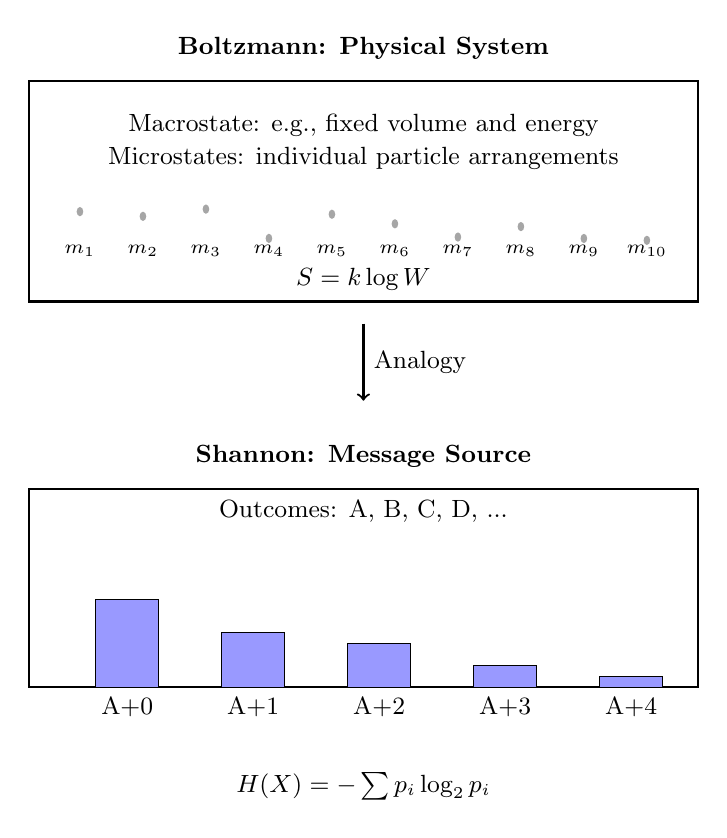
\begin{tikzpicture}[scale=1, every node/.style={font=\small}, yscale=1.4]

% Boltzmann Block (Top)
\draw[thick] (-4.25,8) rectangle (4.25,10);
\node at (0,10.3) {\textbf{Boltzmann: Physical System}};
\node at (0,9.6) {\small Macrostate: e.g., fixed volume and energy};
\node at (0,9.3) {\small Microstates: individual particle arrangements};

% Microstates as labeled dots (spread wider)
\foreach \i/\x in {1/-3.6, 2/-2.8, 3/-2.0, 4/-1.2, 5/-0.4, 6/0.4, 7/1.2, 8/2.0, 9/2.8, 10/3.6} {
    \fill[gray!70] (\x,8.7 + 0.15*rand) circle (1.2pt);
    \node[below] at (\x,8.6) {\scriptsize $m_{\i}$};
}

\node at (0,8.2) {\( S = k \log W \)};

% Connecting Arrow (shortened)
\draw[->, thick] (0,7.8) -- (0,7.1) node[midway, right] {\small Analogy};

% Shannon Block (Bottom)
\draw[thick] (-4.25,4.5) rectangle (4.25,6.3);
\node at (0,6.6) {\textbf{Shannon: Message Source}};
\node at (0,6.1) {\small Outcomes: A, B, C, D, ...};

% Centered bar chart in Shannon block (shifted left slightly)
\foreach \i/\p in {0/0.4, 1/0.25, 2/0.2, 3/0.1, 4/0.05} {
    \pgfmathsetmacro{\xstart}{-3.4 + \i*1.6}
    \draw[fill=blue!40] (\xstart,4.5) rectangle +(.8,\p*2);
    \node[below] at (\xstart + 0.4,4.5) {\char65+\i}; % A, B, C, D, E
}

% Shannon entropy equation (moved further down)
\node at (0,3.6) {\( H(X) = -\sum p_i \log_2 p_i \)};

\end{tikzpicture}
\caption{
\textbf{Two kinds of entropy, one deep idea.} Boltzmann entropy (top) counts the number of microstates (\( m_1, m_2, \dots \)) that correspond to a single macrostate like volume or energy. Shannon entropy (bottom) measures the uncertainty in a probabilistic message source. The less predictable the outcome, the more information is gained once a symbol is chosen.
}
\end{figure}










Shannon’s genius was to treat messages the way physicists treated molecules—statistical ensembles governed by probability distributions. And just as Boltzmann’s entropy told us what configurations were likely, Shannon’s entropy told us how efficiently we could encode and transmit data drawn from those distributions.

This unification didn’t arise in a vacuum. In the early 20th century, \textbf{Andrey Kolmogorov} had already revolutionized probability by tying it to \textbf{measure theory}—the same mathematical framework used in Lebesgue integration. Kolmogorov’s formalism made it possible to treat probabilities not as hand-wavy guesses, but as measurable structures on a space of outcomes.

With this foundation in place, Shannon’s entropy became more than a metaphor. It was a rigorous quantity—a measure over a probability space. And once you had a measure, you could integrate. You could optimize. You could build systems.

Even \textbf{Fourier analysis}, originally developed to study the flow of heat, reappeared here. Just as Fourier decomposed waveforms into simpler frequencies, information theory decomposes uncertainty into bits. Where Boltzmann counted states, Kolmogorov measured spaces, and Fourier captured structure—Shannon brought it all together.

And so, entropy—once a tool to analyze steam engines—became the cornerstone of modern communication, data compression, cryptography, and machine learning.

From thermodynamic disorder to digital uncertainty, the math is the same. Entropy tells us not just how disordered or uncertain something is—but how much can be known, encoded, or lost.

\begin{quote}
In the end, every bit is a question. Every question reduces uncertainty. And every answer—that’s information.
\end{quote}




\begin{tcolorbox}[title={\textbf{Historical Sidebar: The Medium as Encoder and Decoder}}, colback=gray!5, colframe=black, fonttitle=\bfseries]

  Before Shannon formalized information theory, the dominant view of communication focused on \textbf{content}: the meaning of a message, the truth of a statement, the clarity of the words. But in 1964, philosopher and media theorist \textbf{Marshall McLuhan} flipped this logic on its head with a provocative claim: \textit{“The medium is the message.”}
  
  \medskip
  
  In system-theoretic terms, every medium -- whether radio waves, paper, silicon, or neurons -- \textbf{constrains} how signals are structured, transmitted, and interpreted. A signal is never “just” its content; the medium shapes the signal.

  \medskip

  In other words: \textbf{No signal is just data since the method of transmission alters what the system perceives.}

  \medskip
  
  \begin{itemize}

    \item A \textbf{serial bus} and a \textbf{parallel bus} deliver the same bits, but demand different hardware assumptions.
    \item Even if the payload is identical, a \textbf{real-time stream} versus a \textbf{batch transmission} invokes different processing paradigms.
    \item \textbf{Analog} and \textbf{digital} signals can encode equivalent content, but have completely different filtering, sampling, and decoding behaviors.
  \end{itemize}
  
  \medskip
  
  In this view, the \textbf{medium acts as both encoder and decoder}. The medium determines what messages can exist and what they can mean in a system. A low-bandwidth medium biases toward compression. A noisy channel prioritizes redundancy. A lossy medium alters which bits matter most.
  
  \begin{quote}
  Every signal carries metadata in its medium. And every system reacts not just to the message, but to the way the message arrives.
  \end{quote}
  
\end{tcolorbox}

  
  
  
  






\subsection{From Molecules to Messages: Shannon’s Unification of Physics and Information}

Claude Shannon’s breakthrough was more than just clever engineering. It was a conceptual unification—a fusion of physics, probability, and signal analysis. He didn’t invent the idea of entropy; that credit belongs to Boltzmann. Nor did he invent measure theory—that was Kolmogorov’s domain. And Fourier had been decomposing heat into sine waves long before radios were a twinkle in Maxwell’s equations.

But Shannon connected them all. Let’s break it down.

\subsubsection{Step 1: The Signal as a Function}
In the physical world, we often start with a continuous signal—say, a sound wave or voltage over time. Mathematically, this is just a function \( f(t) \), defined over a continuous interval.

\begin{figure}[H]
\centering
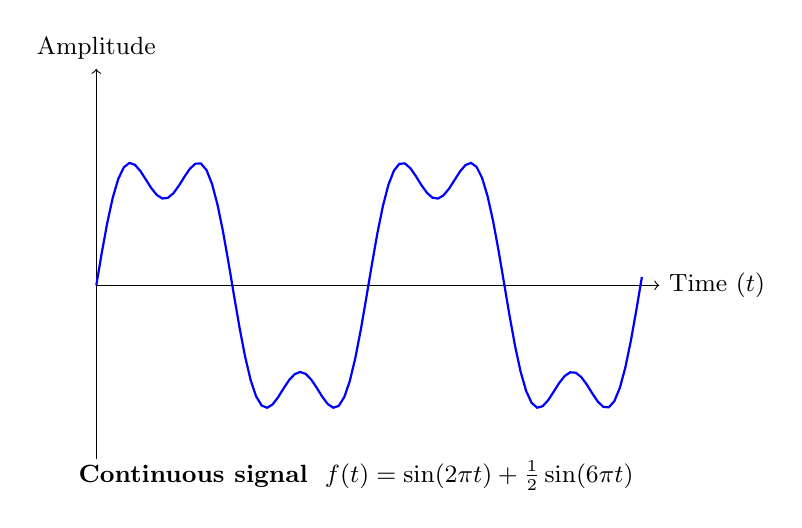
\begin{tikzpicture}[scale=1.1]
  \draw[->] (0,0) -- (6.5,0) node[right] {\small Time ($t$)};
  \draw[->] (0,-2) -- (0,2.5) node[above] {\small Amplitude};

  \draw[thick, blue, domain=0:6.3, samples=100] plot (\x, {1.5*sin(2*\x r) + 0.5*sin(6*\x r)});

  \node[align=center] at (3,-2.2) {\small \textbf{Continuous signal} \ \( f(t) = \sin(2\pi t) + \frac{1}{2} \sin(6\pi t) \)};
\end{tikzpicture}
\caption{A real-world signal: continuous in time, infinitely precise, and impossible to store or transmit directly.}
\end{figure}

In thermodynamics, this function might represent temperature. In communications, it’s a waveform. But either way, it’s rich with infinite detail—and that’s a problem for transmission.

\subsubsection{Step 2: Sampling and Discretization}
Shannon realized that if the signal is \emph{bandlimited}—meaning it contains no frequencies above a certain threshold—then we don’t need the entire curve. Just sample it at regular intervals.

\begin{figure}[H]
\centering
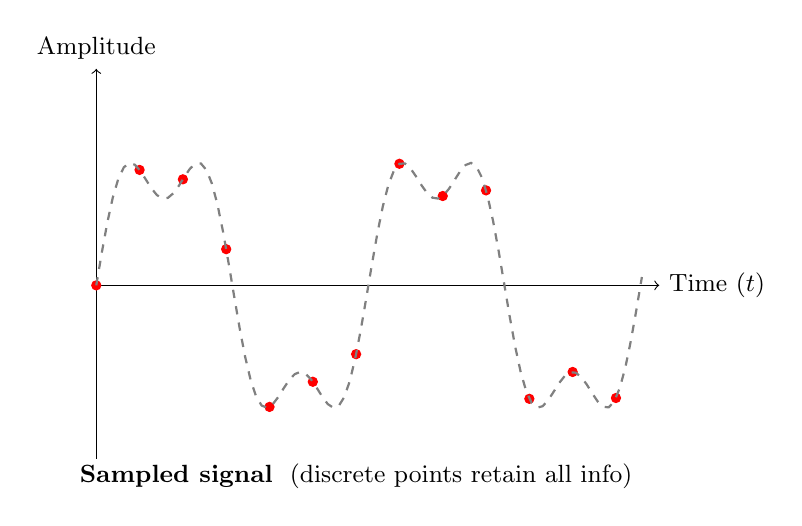
\begin{tikzpicture}[scale=1.1]
  \draw[->] (0,0) -- (6.5,0) node[right] {\small Time ($t$)};
  \draw[->] (0,-2) -- (0,2.5) node[above] {\small Amplitude};

  \foreach \x in {0,...,12} {
    \pgfmathsetmacro\val{1.5*sin(2*deg(0.5*\x)) + 0.5*sin(6*deg(0.5*\x))}
    \filldraw[red] ({0.5*\x}, \val) circle (1.5pt);
  }

  \draw[thick, dashed, gray, domain=0:6.3, samples=100] plot (\x, {1.5*sin(2*\x r) + 0.5*sin(6*\x r)});

  \node[align=center] at (3,-2.2) {\small \textbf{Sampled signal} \ (discrete points retain all info)};
\end{tikzpicture}
\caption{According to Shannon’s sampling theorem, a bandlimited signal can be reconstructed from discrete samples.}
\end{figure}

Here, measure theory enters the chat. Kolmogorov’s axioms let us treat the space of samples probabilistically: each sample becomes a random variable, drawn from a distribution with structure and meaning.

\subsubsection{Step 3: Decomposition via Fourier and Entropy}
Now we take those samples and decompose them. Fourier’s gift was to show that any signal could be written as a sum of sinusoids. Each frequency is a microstate. The more frequencies, the more uncertainty about what the signal is doing next.

\begin{figure}[H]
\centering
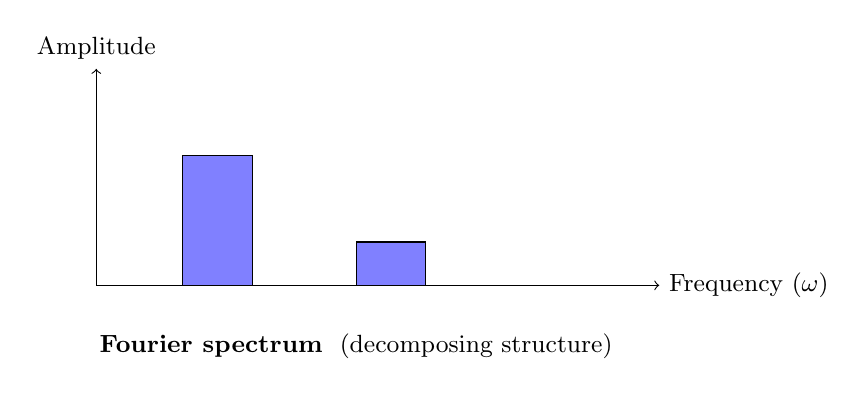
\begin{tikzpicture}[scale=1.1]
  \draw[->] (0,0) -- (6.5,0) node[right] {\small Frequency ($\omega$)};
  \draw[->] (0,0) -- (0,2.5) node[above] {\small Amplitude};

  % Fourier bars
  \foreach \x/\h in {1/1.5, 3/0.5} {
    \draw[fill=blue!50] (\x,0) rectangle +(0.8,\h);
  }

  \node[align=center] at (3,-0.7) {\small \textbf{Fourier spectrum} \ (decomposing structure)};
\end{tikzpicture}
\caption{Fourier analysis breaks the signal into frequencies—each a possible microstate. More frequencies = more entropy.}
\end{figure}

This is where Shannon’s entropy kicks in:
\[
H(X) = - \sum_i p_i \log_2 p_i
\]
Each frequency’s amplitude becomes a probability weight. Entropy tells us how uncertain—or how compressible—the signal really is.


\subsubsection{Step 4: The Power Spectrum — Energy as Structure}

Why decompose a function into frequencies? Because real-world signals—whether they’re sound waves, electrical currents, or stock market fluctuations—are rarely pure sine waves. They’re messy, layered, and complex. Decomposing a signal into its frequency components reveals what it’s truly made of.

This decomposition gives us more than just insight—it gives us the **power spectrum**.

\begin{figure}[H]
\centering
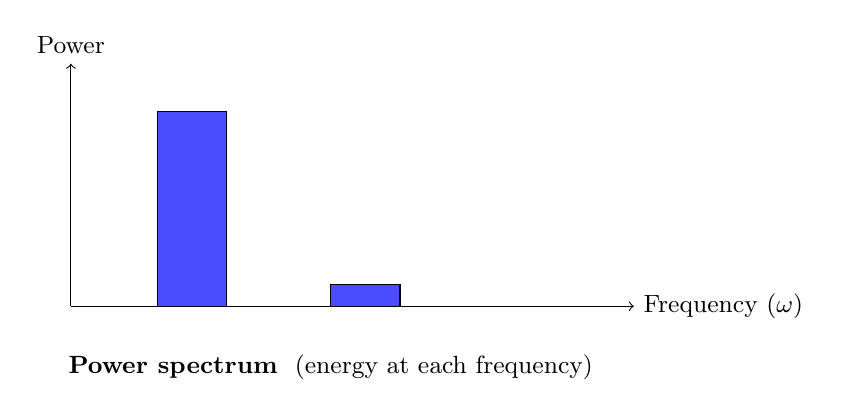
\begin{tikzpicture}[scale=1.1]
  \draw[->] (0,0) -- (6.5,0) node[right] {\small Frequency ($\omega$)};
  \draw[->] (0,0) -- (0,2.8) node[above] {\small Power};

  % Power spectrum bars
  \foreach \x/\h in {1/2.25, 3/0.25} {
    \draw[fill=blue!70] (\x,0) rectangle +(0.8,\h);
  }

  \node[align=center] at (3,-0.7) {\small \textbf{Power spectrum} \ (energy at each frequency)};
\end{tikzpicture}
\caption{The power spectrum shows where the energy lives. Peaks represent dominant frequencies.}
\end{figure}

Each bar tells us how much **energy** is contained in a given frequency. High bars? Dominant components. Low bars? Background noise. This is where the physics kicks in: energy is conserved, but how it’s distributed determines how predictable—or unpredictable—the signal is.

And that’s where entropy returns.

Entropy measures how spread out the energy is across frequencies. If all the power is in one frequency, the entropy is low—there’s order. But if the power is smeared across many frequencies, entropy increases. The signal becomes more complex, less compressible, more uncertain.

In essence:
\begin{itemize}
  \item The power spectrum maps **energy**.
  \item Entropy maps **uncertainty**.
  \item When energy spreads, so does entropy.
\end{itemize}

This deep connection is what Shannon inherited from Boltzmann: whether we're looking at heat in molecules or structure in messages, **energy and entropy are two sides of the same informational coin**.


\subsubsection{Putting It All Together}

What Boltzmann did for gas molecules, Shannon did for messages. Both realized that uncertainty—whether physical or informational—follows the same mathematical logic. 

When we decompose a signal, we’re not just cleaning up noise—we’re mapping how **energy** flows across **structure**. Each frequency carries a portion of that energy, and the **spread** of energy across those frequencies is what generates **entropy**.

\begin{itemize}
  \item Break the signal into components (Fourier modes, letters, or states)
  \item Measure where the energy goes
  \item Apply entropy to understand uncertainty and compressibility
\end{itemize}


\begin{figure}[H]
\centering
\begin{tikzpicture}[>=latex, every node/.style={font=\footnotesize}, scale=1.1]

% Top Row
\node[draw, thick, rounded corners=2pt, fill=blue!10, minimum width=4cm, minimum height=1.5cm] (signal) at (0,0) {
  \begin{tabular}{c}
    \textbf{Signal} \\[0.2em]
    $f(t) = \sin(2\pi t) + \frac{1}{2} \sin(6\pi t)$
  \end{tabular}
};

\node[draw, thick, rounded corners=2pt, fill=green!10, minimum width=4.5cm, minimum height=1.5cm, right=4.2cm of signal] (spectrum) {
  \begin{tabular}{c}
    \textbf{Power Spectrum} \\[0.2em]
    Energy by frequency \\ (e.g., bar heights at $\omega_1$, $\omega_2$)
  \end{tabular}
};

% Bottom Row
\node[draw, thick, rounded corners=2pt, fill=purple!10, minimum width=4.2cm, minimum height=1.5cm, below=2.2cm of signal] (interpretation) {
  \begin{tabular}{c}
    \textbf{Interpretation} \\[0.2em]
    Does the decomposition reveal \\ patterns, predictions, compression?
  \end{tabular}
};

\node[draw, thick, rounded corners=2pt, fill=orange!10, minimum width=4.2cm, minimum height=1.5cm, below=2.2cm of spectrum] (entropy) {
  \begin{tabular}{c}
    \textbf{Entropy} \\[0.2em]
    $H(X) = -\sum p_i \log_2 p_i$
  \end{tabular}
};

% Arrows
\draw[->, thick] (signal) -- node[above, font=\footnotesize, yshift=0.2em] {Decompose into components} (spectrum);
\draw[->, thick] (spectrum) -- node[left, font=\footnotesize, xshift=0.3em] {Measure energy spread} (entropy);
\draw[->, thick] (signal) -- node[right, font=\footnotesize, xshift=-0.3em] {Guiding question} (interpretation);
\draw[->, thick] (entropy) -- node[below, font=\footnotesize, yshift=-0.2em] {Extract insight / action} (interpretation);

% Caption under grid
\node[align=center, font=\footnotesize] at (spectrum |- entropy.south) [yshift=-1.3cm] {
  Decomposition enables measurement.\\
  Measurement reveals uncertainty.\\
  Entropy quantifies uncertainty.\\
  Interpretation brings it all back to meaning.
};

\end{tikzpicture}
\caption{A full cycle: from raw signal to structure, entropy, and back to meaning.}
\end{figure}



After all the math, this is what the pipeline really means:

We begin with a \textbf{signal}—a voltage trace, a stock price curve, a chunk of audio—and a \textbf{question}:

\begin{quote}
\textit{Is there structure here?}
\end{quote}

To answer that, we \textbf{decompose} the signal. Fourier analysis, wavelets, Z-transforms, PCA—these tools help us express the signal in terms of \textbf{basis components}. This lets us \textbf{measure where the energy lives}.

Then we apply \textbf{entropy}, not just as a formula, but as a lens:

\begin{quote}
\textit{How spread out is the energy? How much structure do we retain? How compressible is the result?}
\end{quote}

Finally, we interpret. Not every signal with high entropy is noise—sometimes it’s complexity. And not every low-entropy signal is simple—sometimes it’s redundancy. Entropy doesn’t just quantify uncertainty; it challenges us to explain it.

\begin{tcolorbox}[title={\textbf{Historical Sidebar: 42, Entropy, and the Problem of Interpretation}}, colback=gray!5, colframe=black, fonttitle=\bfseries]

  In Douglas Adams’ 1979 sci-fi classic \textit{The Hitchhiker’s Guide to the Galaxy}, a race of hyper-intelligent beings builds a computer—\textbf{Deep Thought}—to answer the ultimate question of life, the universe, and everything. After seven and a half million years of computation, Deep Thought solemnly replies: \textbf{42}.

  \medskip
  
  The problem? No one understands the answer.

  \medskip
  
  This is not just absurdist humor: it’s a parable for information theory.  Entropy tells us how much uncertainty a signal resolves, but it says nothing about what the signal \textit{means}.
 
  \begin{quote}
  
  Ultimately, nobody understood the answer because nobody understood the question. 

  \end{quote}
  
  The moral? Without a shared interpretive framework, all messages are just bits in the void; so, if you don’t understand what you are asking then even the perfect answer won’t make sense.
  
\end{tcolorbox}
  
\subsection{From Concept to Practice: How Decomposition Shapes Interpretation}

Let’s say we’re analyzing a noisy, repeating sawtooth wave. 

\begin{figure}[H]
\centering
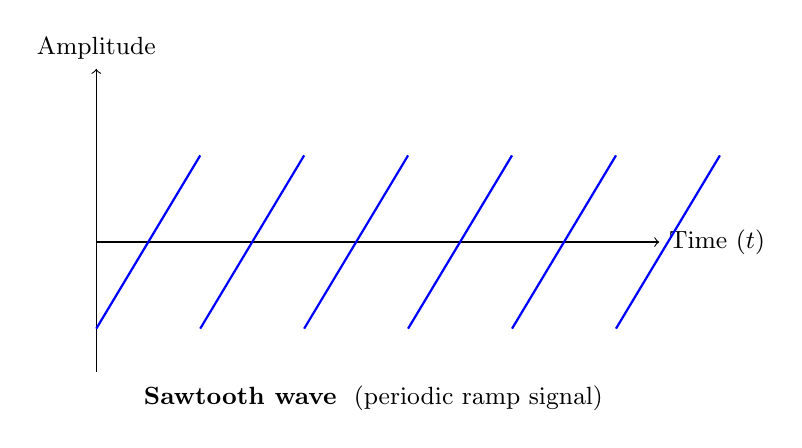
\begin{tikzpicture}[scale=1.1]
  % Axes
  \draw[->] (0,0) -- (6.5,0) node[right] {\small Time ($t$)};
  \draw[->] (0,-1.5) -- (0,2) node[above] {\small Amplitude};

  % Sawtooth wave
  \foreach \x in {0,...,5} {
    \draw[thick, blue] ({\x*1.2}, -1) -- ({(\x+1)*1.2}, 1);
  }

  % Optional: simulated noise (tiny random bumps)
  % \foreach \x in {0,...,60} {
  %   \pgfmathsetmacro\noise{rand*0.3 - 0.15}
  %   \pgfmathsetmacro\t{0.13*\x}
  %   \pgfmathsetmacro\val{2*mod(\t,1.2)/1.2 - 1 + \noise}
  %   \fill[red] (\t, \val) circle (0.4pt);
  % }

  % Label
  \node[align=center] at (3.2,-1.8) {\small \textbf{Sawtooth wave} \ (periodic ramp signal)};
\end{tikzpicture}
\caption{A basic sawtooth wave: rises linearly and resets. Useful for modeling periodic, discontinuous systems.}
\end{figure}


How we decompose the same signal with different methods changes what we learn:

\begin{quote}
\textbf{different decomposition = different entropy = different insight.} 
\end{quote}

The method we choose shapes what we can see, and what we can compress.

\begin{figure}[H]
\centering
\begin{tikzpicture}[>=latex, every node/.style={font=\footnotesize}, scale=1]

% Fourier and Wavelet side by side
\node[draw, thick, rounded corners=2pt, fill=green!10, minimum width=4.2cm, minimum height=1.2cm] (fourier) at (-3,0) {
  \begin{tabular}{c}
    \textbf{Fourier Transform} \\[0.2em]
    Spread across many \\ global sinusoids
  \end{tabular}
};

\node[draw, thick, rounded corners=2pt, fill=purple!10, minimum width=4.2cm, minimum height=1.2cm] (wavelet) at (3,0) {
  \begin{tabular}{c}
    \textbf{Wavelet Transform} \\[0.2em]
    Localized, sparse \\ representation
  \end{tabular}
};

% Input Signal (centered above)
\node[draw, thick, rounded corners=2pt, fill=blue!10, minimum width=5cm, minimum height=1.2cm, above=2.1cm of $(fourier)!0.5!(wavelet)$] (signal) {
  \begin{tabular}{c}
    \textbf{Input Signal} \\[0.2em]
    Noisy sawtooth wave
  \end{tabular}
};

% Arrows from center bottom of signal box with shifted labels
\draw[->, thick] (signal.south) to[bend right=15] node[below left=6pt, xshift=-1.5em] {\footnotesize Fourier path} (fourier.north);
\draw[->, thick] (signal.south) to[bend left=15] node[below right=6pt, xshift=1.5em] {\footnotesize Wavelet path} (wavelet.north);

% Entropy boxes below each method
\node[draw, thick, rounded corners=2pt, fill=orange!10, minimum width=3.6cm, minimum height=1.1cm, below=1.6cm of fourier] (entropyF) {
  \begin{tabular}{c}
    \textbf{Entropy: High} \\[0.2em]
    Many components active
  \end{tabular}
};

\node[draw, thick, rounded corners=2pt, fill=orange!10, minimum width=3.6cm, minimum height=1.1cm, below=1.6cm of wavelet] (entropyW) {
  \begin{tabular}{c}
    \textbf{Entropy: Low} \\[0.2em]
    Fewer components active
  \end{tabular}
};

% Arrows from methods to entropy
\draw[->, thick] (fourier) -- (entropyF);
\draw[->, thick] (wavelet) -- (entropyW);

% Caption
\node[align=center, font=\footnotesize] at (0,-4.5) {
  Same signal, different decompositions: Fourier spreads energy, wavelets concentrate it.\\
  Entropy measures how much structure—or randomness—we’ve captured.
};

\end{tikzpicture}
\caption{Comparing decomposition approaches: global vs. localized, spread vs. sparse.}
\end{figure}


\vspace{1em}
\subsubsection*{Zooming In: What Do the Transforms Actually Show?}

The method we choose shapes what we can see, and what we can compress.

The \textbf{Fourier Transform} breaks a signal into a sum of sinusoids. It tells us which frequencies are present and how much energy each one carries. It’s ideal when we’re interested in overall periodic structure—like the presence of regular oscillations.

The \textbf{Z-Transform}, on the other hand, is built for discrete signals and recursive systems—ones where each step depends on the past. Instead of just measuring frequency content, it tells us how the system evolves over time. It reveals repeating patterns that depend on history, delay, or feedback.

Both transforms can produce a \textbf{power spectrum}, but they focus on different kinds of structure.

\vspace{1em}

\begin{figure}[H]
\centering
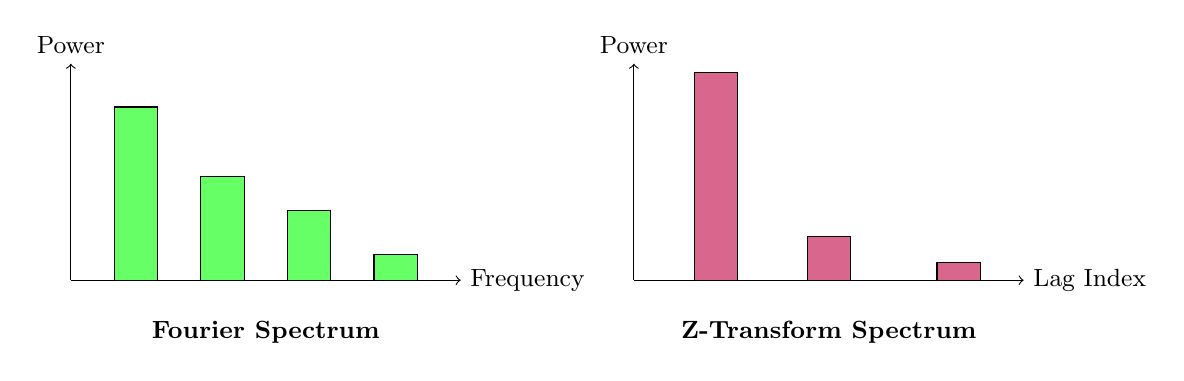
\begin{tikzpicture}[scale=1.1]

% Axes for Fourier
\begin{scope}
  \draw[->] (0,0) -- (4.5,0) node[right] {\small Frequency};
  \draw[->] (0,0) -- (0,2.5) node[above] {\small Power};

  % Fourier bars
  \foreach \x/\h in {0.5/2, 1.5/1.2, 2.5/0.8, 3.5/0.3} {
    \draw[fill=green!60] (\x,0) rectangle +(0.5,\h);
  }

  \node[align=center] at (2.25,-0.6) {\small \textbf{Fourier Spectrum}};
\end{scope}

% Axes for Z-transform (shifted right)
\begin{scope}[xshift=6.5cm]
  \draw[->] (0,0) -- (4.5,0) node[right] {\small Lag Index};
  \draw[->] (0,0) -- (0,2.5) node[above] {\small Power};

  % Z-transform bars (e.g., sharper peaks)
  \foreach \x/\h in {0.7/2.4, 2.0/0.5, 3.5/0.2} {
    \draw[fill=purple!60] (\x,0) rectangle +(0.5,\h);
  }

  \node[align=center] at (2.25,-0.6) {\small \textbf{Z-Transform Spectrum}};
\end{scope}

\end{tikzpicture}
\caption{Power spectra from different transforms. Fourier highlights frequency content; Z-transform reveals effects of delay, recursion, and time-evolving structure.}
\end{figure}


\vspace{1em}
\subsubsection{How Interpretation Depends on the Method}

Each transformation tells a different story about the same signal.

The \textbf{Fourier Transform} frames the signal in terms of how much it "resonates" at each frequency. Interpreting the spectrum means asking:  
> \textit{Which frequencies dominate the behavior of this signal over time?}

A sharp peak at a low frequency suggests slow, steady oscillations. A wide spread implies richer or more erratic structure. From this view, the signal is treated like sound or vibration: energy is organized by frequency.

The \textbf{Z-Transform}, by contrast, invites a different interpretation. It focuses on how the signal evolves step by step, especially when past values influence the future. When we interpret a Z-spectrum, we ask:  
> \textit{How much does each past state contribute to what comes next?}

A strong peak at a particular lag index might mean the system has memory or feedback. Instead of pure tones, we’re now thinking in terms of dynamic structure—like a digital filter or a time-series model.

\medskip

\noindent
\textbf{Same signal, different tools, different questions:}

\begin{itemize}
  \item Fourier asks: \textit{“What is this made of?”}
  \item Z-Transform asks: \textit{“How is this behaving over time?”}
\end{itemize}

Choosing a method is more than a technical step—it frames what you’re able to see, and what kind of explanation you’re allowed to give.

\begin{tcolorbox}[title={\textbf{Historical Footnote: The Perils of Mismatched Decoding}}, colback=gray!5, colframe=black, fonttitle=\bfseries]

  In telecommunications, the phenomenon known as \textbf{falsing} illustrates the importance of aligning decoding methods with the original encoding scheme. Falsing occurs when a system mistakenly interprets unintended signals as valid inputs—often because the decoder applies the wrong interpretive model to the signal.

  \medskip
  
  For example, tone-based signaling systems (such as in early telephone networks) sometimes misfired when a decoder picked up harmonics or noise and interpreted them as legitimate dial tones. One case involved a telephone answering machine erroneously detecting pulse signals from a rotary phone as a ring tone—causing it to answer calls unexpectedly.

  \medskip
  
  Such mismatches between encoding and decoding don't just lead to technical malfunctions—they also render any measure of entropy \emph{misleading}. Entropy only captures uncertainty accurately \textbf{if the decoder's model matches the encoder's}. When that alignment breaks, the system can no longer reliably measure or manage information.
  
\end{tcolorbox}



\subsection{When Sampling Assumes Measurability}

The success of Shannon’s sampling theorem depends on more than clever mathematics—it depends on a certain kind of universe. One where signals are well-behaved, where integration makes sense, and where “measuring something” actually means something.

At the heart of this is measurability.

A signal, after all, is just a function. But for it to be useful—something we can digitize, manipulate, or reconstruct—it has to live in a space with structure:

\begin{itemize}
  \item Where we can define the \textbf{average value} of a signal over an interval.
  \item Where we can talk about \textbf{energy} and \textbf{frequency content} in a rigorous way.
  \item Where sets have a defined \textbf{length}, and functions have a meaningful \textbf{integral}.
  \item Where transformations converge, and limits behave.
\end{itemize}

In other words: a signal must be part of a measurable framework—typically a function in \( L^2(\mathbb{R}) \), the space of square-integrable functions with respect to Lebesgue measure.

This is what allows us to say:
\[
f(t) = \sum_{n=-\infty}^{\infty} f(nT) \cdot \text{sinc}\left(\frac{t - nT}{T}\right)
\]
and actually mean it.

If a signal lies in such a space, then we can apply Shannon’s theorem with full confidence. We can sample it at discrete points, reconstruct it perfectly, and know that the energy it carries is preserved in the process. The signal is smooth enough to analyze, and structured enough to compress. Everything fits.

\begin{quote}
\textbf{All functions are reconstructible—with enough bandwidth—\emph{provided} the underlying structure supports measure.}
\end{quote}

This assumption is so deeply baked into our tools that we rarely question it. But it is an assumption.

Sampling assumes that the signal lives on a space where lengths can be assigned, integrals can be evaluated, and subsets can be compared in size. It assumes that the signal “makes sense” in a world governed by continuity and measure.

If that assumption fails, everything else follows.

\medskip

\noindent
For now, everything seems stable. But we’ll soon ask: what happens when a function exists, but no longer behaves?

When we can’t assign it an average.  
When we can’t sample it.  
When we can’t even measure the set it lives on.

That’s when the cracks begin to show.




\subsection{Revisiting the Dirichlet Function: A Structured System with No Structure?}

Earlier, we met the Dirichlet function—a seemingly simple mathematical object defined as 1 on rational numbers and 0 on irrationals. It’s easy to describe, easy to write down, and perfectly deterministic. And yet, it breaks nearly every tool we’ve built.

It’s discontinuous everywhere. It’s not Riemann-integrable. And when we try to apply Fourier analysis, it refuses to yield. The function has no smoothness, no periodic behavior, no decaying frequency components.

So here’s the dilemma:

\begin{quote}
How can something so precisely defined contain so little usable structure?
\end{quote}

Up to this point, we’ve looked at structure through the lens of probability, measure, and information. Now we bring in energy—how a function’s intensity is distributed—and use it to explain why certain transformations succeed or fail.

With this perspective, we can revisit the Dirichlet function not just as a pathological edge case, but as a signal with **maximum disorder**—a kind of entropy explosion that spills across every frequency.

Let’s see what that actually looks like.









\subsubsection{When Energy Fails: The Fourier Breakdown of Irregularity}

Up until now, we’ve seen how entropy gave us a way to quantify uncertainty, structure, and compressibility—whether in thermodynamic systems, probabilistic models, or communication signals. We explored how Fourier analysis decomposes complex signals into fundamental frequencies, how Lebesgue measure allowed us to rigorously assign weight to irregular sets, and how Shannon tied it all together to formalize the flow of information.

But what happens when none of this structure behaves nicely?

Enter the Dirichlet function: defined as 1 for rational numbers and 0 for irrationals. It’s discontinuous everywhere, and unmeasurable in the Riemann sense. As we now understand through Kolmogorov and Lebesgue, it's measurable—but barely usable.

So how do we understand why Fourier analysis fails for such functions?

Let’s turn to energy.

\[
E(f) = \int_{-\pi}^{\pi} |f(x)|^2 \,dx
\]

This expression—familiar from signal processing—gives the total “energy” of a function over a domain. Think of it as a way to measure how intense or oscillatory a function is. And here’s the crucial link to Fourier theory: via Parseval’s theorem, this energy can be broken down into contributions from each frequency:

\[
E(f) = \sum_{n=0}^{\infty} \left( \frac{a_n^2}{2} + \frac{b_n^2}{2} \right)
\]

This tells us something profound: for Fourier analysis to reconstruct a function meaningfully, its energy must be well-distributed across its harmonic components.

\begin{itemize}
    \item For smooth, well-behaved functions—like the continuous signals Shannon envisioned—this energy tapers off with higher frequencies.
    \item The Fourier coefficients decay, the energy converges, and reconstruction is possible.
\end{itemize}

\begin{center}
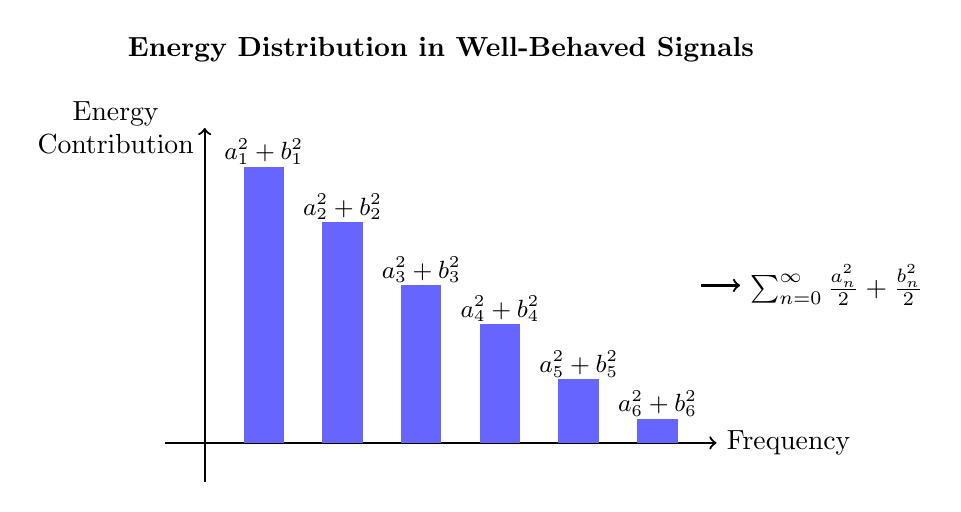
\begin{tikzpicture}
    \draw[thick,->] (-0.5,0) -- (6.5,0) node[right] {Frequency};
    \draw[thick,->] (0,-0.5) -- (0,4) node[left] {\parbox{2cm}{\centering Energy \\ Contribution}};

    \filldraw[blue!60] (0.5,3.5) rectangle (1.0,0);
    \filldraw[blue!60] (1.5,2.8) rectangle (2.0,0);
    \filldraw[blue!60] (2.5,2.0) rectangle (3.0,0);
    \filldraw[blue!60] (3.5,1.5) rectangle (4.0,0);
    \filldraw[blue!60] (4.5,0.8) rectangle (5.0,0);
    \filldraw[blue!60] (5.5,0.3) rectangle (6.0,0);

    \node at (0.75,3.7) {\small \( a_1^2 + b_1^2 \)};
    \node at (1.75,3.0) {\small \( a_2^2 + b_2^2 \)};
    \node at (2.75,2.2) {\small \( a_3^2 + b_3^2 \)};
    \node at (3.75,1.7) {\small \( a_4^2 + b_4^2 \)};
    \node at (4.75,1.0) {\small \( a_5^2 + b_5^2 \)};
    \node at (5.75,0.5) {\small \( a_6^2 + b_6^2 \)};

    \draw[thick, ->] (6.3,2) -- (6.8,2) node[right] {\(\sum_{n=0}^{\infty} \frac{a_n^2}{2} + \frac{b_n^2}{2}\)};
    \node at (3,5.0) {\textbf{Energy Distribution in Well-Behaved Signals}};
\end{tikzpicture}
\end{center}

This graph breaks down a function’s energy into its individual frequency components, giving us a power spectrum. Why do this? Because signals—whether they’re sound waves, electrical currents, or even stock market fluctuations—are rarely just one simple wave. Instead, they’re made up of many different frequencies combined together. The x-axis (Frequency) tells us how fast each of these components oscillates, while the y-axis (Energy Contribution) tells us how much of the total signal's energy comes from each frequency. This breakdown is useful in everything from audio processing (identifying sound patterns), to radio transmission (filtering signals), to medical imaging (reconstructing MRI scans). By understanding how a signal’s energy is spread across frequencies, we can detect patterns, remove unwanted noise, and even reconstruct missing information—all thanks to Fourier’s insights.

But for pathological functions—like Dirichlet’s—the coefficients don’t behave. They don’t decay. They don't even converge meaningfully. The result?

\begin{itemize}
    \item Energy appears chaotically scattered across infinitely many frequencies.
    \item There’s no dominant structure—just noise.
    \item Fourier reconstruction fails not due to philosophical limits, but due to physical incoherence.
\end{itemize}

\begin{figure}[H]
    \centering
    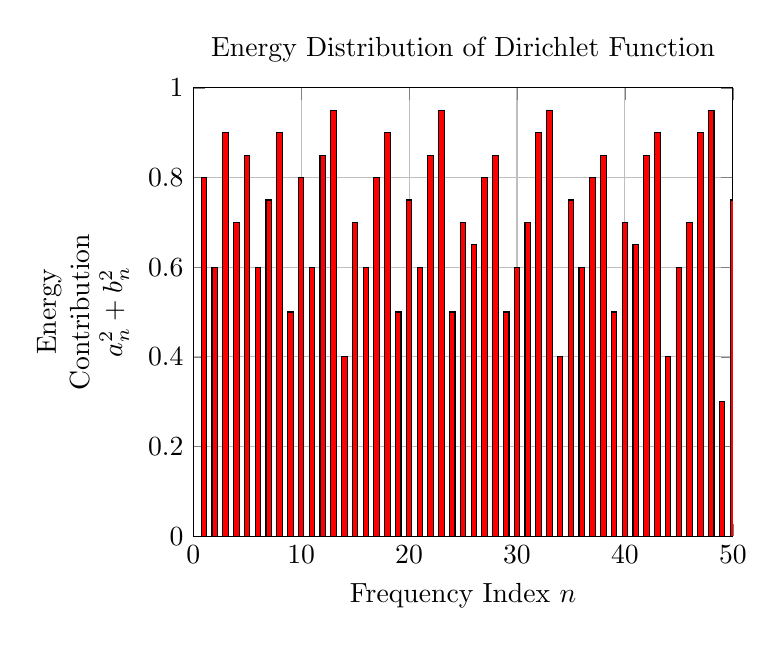
\begin{tikzpicture}
        \begin{axis}[
            title={Energy Distribution of Dirichlet Function},
            xlabel={Frequency Index \( n \)},
            ylabel={\parbox{2cm}{\centering Energy \\ Contribution \\ \( a_n^2 + b_n^2 \)}},
            xmin=0, xmax=50,
            ymin=0, ymax=1,
            xtick={0,10,20,30,40,50},
            ytick={0,0.2,0.4,0.6,0.8,1},
            grid=major,
            domain=1:50
        ]
            % Erratic energy distribution with non-decaying values as bars
            \addplot[ybar, fill=red, bar width=2pt] 
            coordinates {
                (1, 0.8) (2, 0.6) (3, 0.9) (4, 0.7) (5, 0.85) 
                (6, 0.6) (7, 0.75) (8, 0.9) (9, 0.5) (10, 0.8)
                (11, 0.6) (12, 0.85) (13, 0.95) (14, 0.4) (15, 0.7)
                (16, 0.6) (17, 0.8) (18, 0.9) (19, 0.5) (20, 0.75)
                (21, 0.6) (22, 0.85) (23, 0.95) (24, 0.5) (25, 0.7)
                (26, 0.65) (27, 0.8) (28, 0.85) (29, 0.5) (30, 0.6)
                (31, 0.7) (32, 0.9) (33, 0.95) (34, 0.4) (35, 0.75)
                (36, 0.6) (37, 0.8) (38, 0.85) (39, 0.5) (40, 0.7)
                (41, 0.65) (42, 0.85) (43, 0.9) (44, 0.4) (45, 0.6)
                (46, 0.7) (47, 0.9) (48, 0.95) (49, 0.3) (50, 0.75)
            };

        \end{axis}
    \end{tikzpicture}
    \caption{Unlike well-behaved functions, the Dirichlet function's Fourier coefficients fail to decay properly, leading to erratic energy distribution across frequencies.}
\end{figure}

This graph attempts to break down the Dirichlet function’s energy into its individual frequency components, just like a power spectrum. Normally, this would help us understand how much of a signal’s energy is stored at different frequencies—useful for everything from sound processing to radio signals to medical imaging. But here’s the problem: this graph is a mess.

In a well-behaved function, we expect to see the energy decay smoothly as frequency increases. This tells us that most of the energy is concentrated in the lower frequencies, making it possible to reconstruct the function efficiently. But for the Dirichlet function? No such luck. Instead of a nice, orderly drop-off, we get erratic, scattered values that don’t settle down—meaning the energy is spread unpredictably across infinitely many frequencies.

The reason the graph uses points instead of a continuous curve is that Fourier series break a function into discrete frequency components, each represented by a separate term. Normally, this would create a meaningful pattern in how energy is distributed. But here, the random-looking spikes tell us something important: there is no dominant frequency structure. The energy is chaotically spread across infinitely many frequencies, making reconstruction meaningless.

This also gives insight into why the integral of the Dirichlet function is zero. Looking at the graph, we see that the energy doesn’t accumulate in any meaningful way—it fluctuates wildly without forming a coherent structure. This reflects how the function itself oscillates erratically between 1 and 0 across its domain. Since positive and negative contributions cancel out on a large scale, the total integral over any continuous interval effectively sums to zero.

In practical applications, this kind of behavior is a nightmare. If we were trying to use this function in audio processing, it wouldn’t sound like a tone or even noise—it would be something completely incoherent. If we were using it in signal transmission, it would be utterly unusable because the signal carries no discernible structure. In short, this function fundamentally breaks the way Fourier analysis is supposed to work, which is why its decomposition is useless in any practical sense.

This brings us full circle.

Entropy, as we saw, is the measure of uncertainty—how widely a distribution is spread across possible outcomes. In a well-structured signal, most of the energy (or probability) is concentrated in a small number of components. That’s what makes compression, reconstruction, and interpretation possible.

But when that spread becomes extreme—when energy is smeared across infinitely many frequencies without meaningful decay—we approach a state that mirrors \emph{maximum entropy}. Not in the strict probabilistic sense, but in its physical analog: total disorder, zero predictability, and no way to recover a coherent signal.

A function like Dirichlet’s isn’t just irregular—it’s the embodiment of what happens when structure collapses. No dominant frequencies. No compressible patterns. Just uniform uncertainty across the board.

And that’s the key insight: 

\begin{quote}
\textit{When you can’t find structure, assume it doesn’t exist. And when nothing is knowable, maximize entropy.}
\end{quote}

This idea isn’t just a fallback—it’s a principled starting point. In the absence of structure, the most honest thing we can do is embrace uncertainty. And that’s exactly what the next section explores.










\subsection{The Principle of Maximum Entropy: What to Assume When You Know Nothing}

Suppose you’ve intercepted a transmission, but you know nothing about the language or its contents. What do you assume? Is every letter equally likely? Are some words more probable than others? Should you guess based on English, or alien Klingon?

This is the dilemma of \emph{maximum ignorance}—and it turns out to be a deeply important question.

In physics, when we don’t know which microstate a system is in, we assume the system is in the \emph{macrostate with the most microstates}. That’s the one most likely to arise by chance. This leads directly to the Second Law of Thermodynamics: left alone, systems tend toward \emph{maximum entropy}.

Shannon realized that the same logic applies to information.

\textbf{When you have no information about a message source, the least biased assumption you can make is the one with maximum entropy.}

That is, you assign probabilities in a way that maximizes uncertainty, subject to whatever constraints you actually do know. No more, no less.

\begin{itemize}
  \item If you know nothing about the outcomes, assume a uniform distribution.
  \item If you know the average value of a signal but nothing else, choose the distribution that maximizes entropy subject to that average.
\end{itemize}

This isn’t just a philosophical posture—it’s a mathematically justified strategy. The resulting distributions often turn out to be familiar:

\begin{itemize}
  \item \textbf{Uniform distribution:} maximum entropy with no constraints.
  \item \textbf{Exponential distribution:} maximum entropy given a fixed mean.
  \item \textbf{Gaussian distribution:} maximum entropy given a fixed mean and variance.
\end{itemize}



Each of these is the most "uninformed" distribution you can choose, given your available knowledge. Anything else smuggles in assumptions.

\begin{quote}
\textbf{Maximum entropy is the art of admitting you don't know something, mathematically.}
\end{quote}

And it leads naturally to our next topic: what happens when you \emph{do} know something?

If entropy is the measure of uncertainty, then \textbf{mutual information} tells us how much that uncertainty gets reduced. It's what happens when a vague guess becomes a calculated prediction—when ambiguity gets replaced by structure.

In short: entropy tells you what you don't know. Mutual information tells you what you learn.











\subsection{From Entropy to Mutual Information: Eliminating Ambiguity}

Imagine you’re trying to guess a password, one letter at a time. If you know absolutely nothing, each guess is pure uncertainty—you’re operating at maximum entropy. But now imagine someone gives you a hint: “It’s an English word, and it starts with ‘T’.” That clue doesn’t tell you the whole password, but it drastically narrows the possibilities.






\begin{figure}[H]
\centering
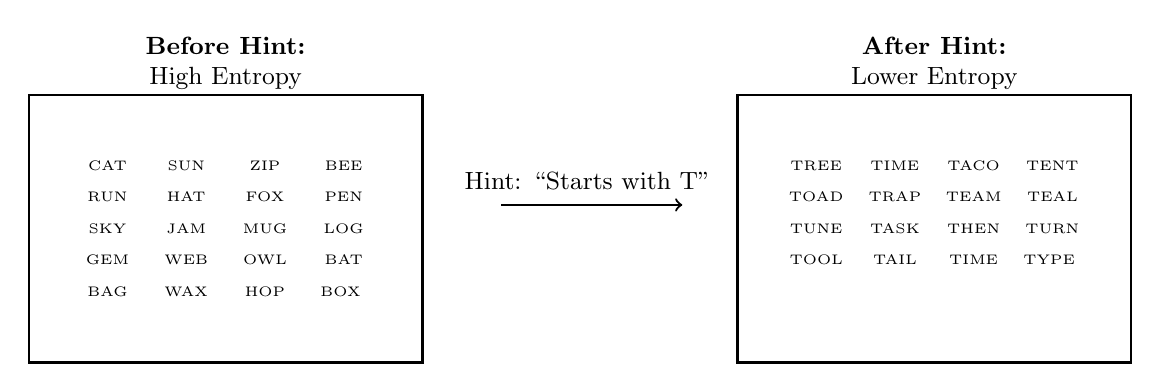
\begin{tikzpicture}[scale=1.0, every node/.style={font=\small}]

% === CONFIGURABLE VARIABLES ===
% Vertical offset for lowering the entire layout
\pgfmathsetmacro{\yoffset}{-2.5}

% Before Hint Grid
\pgfmathsetmacro{\bxstart}{-6.0}
\pgfmathsetmacro{\bystart}{0.5 + \yoffset}
\pgfmathsetmacro{\bxstep}{1.0}
\pgfmathsetmacro{\bystep}{-0.4}

% After Hint Grid
\pgfmathsetmacro{\axstart}{3.0}
\pgfmathsetmacro{\aystart}{0.5 + \yoffset}
\pgfmathsetmacro{\axstep}{1.0}
\pgfmathsetmacro{\aystep}{-0.4}

% === BOXES ===
\draw[thick] (-7, -2 + \yoffset) rectangle (-2, 1.40 + \yoffset);
\node[align=center] at (-4.5,1.8 + \yoffset) {\textbf{Before Hint:} \\ High Entropy};

\draw[thick] (2,-2 + \yoffset) rectangle (7,1.40 + \yoffset);
\node[align=center] at (4.5,1.8 + \yoffset) {\textbf{After Hint:} \\ Lower Entropy};

% === WORDS ===
% Words before hint
\def\beforeWords{
    CAT, SUN, ZIP, BEE,
    RUN, HAT, FOX, PEN,
    SKY, JAM, MUG, LOG,
    GEM, WEB, OWL, BAT,
    BAG, WAX, HOP, BOX
}
\foreach [count=\i] \word in \beforeWords {
    \pgfmathtruncatemacro{\col}{mod(\i-1, 4)}
    \pgfmathtruncatemacro{\row}{int((\i-1)/4)}
    \pgfmathsetmacro{\x}{\bxstart + \col * \bxstep}
    \pgfmathsetmacro{\y}{\bystart + \row * \bystep}
    \node[font=\tiny, align=center] at (\x,\y) {\word};
}

% Words after hint (T-words)
\def\afterWords{
    TREE, TIME, TACO, TENT,
    TOAD, TRAP, TEAM, TEAL,
    TUNE, TASK, THEN, TURN,
    TOOL, TAIL, TIME, TYPE
}
\foreach [count=\i] \word in \afterWords {
    \pgfmathtruncatemacro{\col}{mod(\i-1, 4)}
    \pgfmathtruncatemacro{\row}{int((\i-1)/4)}
    \pgfmathsetmacro{\x}{\axstart + \col * \axstep}
    \pgfmathsetmacro{\y}{\aystart + \row * \aystep}
    \node[font=\tiny, align=center] at (\x,\y) {\word};
}

% Arrow and label
\draw[->, thick] (-1.0,\yoffset) -- (1.3,\yoffset);
\node[align=center] at (0.1,\yoffset + 0.3) {\small Hint: ``Starts with T''};

\end{tikzpicture}

\caption{
\textbf{Left:} Before the hint, the password could be any short English word—uncertainty is high. \\
\textbf{Right:} After receiving a hint (“starts with T”), the set of possible candidates shrinks. The reduced uncertainty is what \emph{mutual information} quantifies. Each box shows the sample space before and after the hint.
}
\end{figure}











This narrowing—the reduction in uncertainty thanks to additional information—is exactly what Claude Shannon quantified with his concept of \textbf{mutual information}.

While entropy measures how uncertain we are about a random variable \( X \), mutual information measures how much that uncertainty drops when we learn something about a related variable \( Y \). If \( Y \) gives us no insight into \( X \), the mutual information is zero. But if knowing \( Y \) fully determines \( X \), the mutual information is as large as the entropy of \( X \) itself.

Formally, Shannon defined it as:
\[
I(X; Y) = H(X) - H(X|Y)
\]
where:
\begin{itemize}
  \item \( H(X) \) is the total uncertainty (entropy) of \( X \),
  \item \( H(X|Y) \) is the remaining uncertainty about \( X \) after observing \( Y \),
  \item \( I(X; Y) \) is the mutual information—the amount of uncertainty eliminated.
\end{itemize}

In simpler terms: mutual information tells us how much knowing \( Y \) helps us guess \( X \).

Let’s say you’re transmitting messages over a noisy channel. You send \( X \), but the receiver hears \( Y \). If the channel is perfect, then \( Y = X \) and all information is preserved. But if the channel is noisy—say, a bad phone connection or an unreliable internet signal—then \( Y \) might be a distorted version of \( X \).

Mutual information quantifies how much of the original message survives the noise.

\begin{itemize}
  \item If \( I(X; Y) = H(X) \), there’s no loss. The channel is ideal.
  \item If \( I(X; Y) = 0 \), the channel is completely noisy; the output \( Y \) tells us nothing about the input \( X \).
\end{itemize}

This idea underpins everything from error-correcting codes to neural networks. It’s how we detect patterns in noisy data, how we compress files without losing essential content, and how we build communication systems that resist interference.

Just like entropy, mutual information relies on the probability distribution over possible outcomes. It assumes we’ve modeled the information source, the transmission process, and the uncertainty involved. And just like entropy, it is deeply geometric: it measures how two sets—representing two random variables—overlap in probability space.

If entropy is the measure of surprise, then mutual information is the measure of understanding. It tells us how much clarity one variable brings to another—how much ambiguity has been removed.

\begin{quote}
In a world filled with noise, mutual information tells us how much signal is left.
\end{quote}

\vspace{1em}
\subsubsection{Example: The Hat Guessing Game and Mutual Information}

Imagine this:

Three logicians are each randomly given a hat—either red or blue. They can all see everyone else’s hats, but not their own. Simultaneously, each person must either:

\begin{itemize}
  \item Guess the color of their own hat (red or blue), or
  \item Pass.
\end{itemize}

If at least one person guesses correctly and no one guesses incorrectly, they all win. If anyone guesses wrong, they all lose. The logicians are allowed to agree on a strategy beforehand, but once the hats are on, no communication is allowed.

Now, each individual lacks full information: they don’t know their own hat color. But collectively, they share some structure—they each see part of the system.

Here’s the clever strategy:

\begin{quote}
Each person assumes that the total number of red hats they see is even. If that assumption leads them to deduce that their own hat must be red, they guess “red.” If it leads them to deduce it must be blue, they guess “blue.” Otherwise, they pass.
\end{quote}

Let’s see why this works. There are 8 total possible hat combinations (RRR, RRB, ..., BBB). For any given combination, exactly \textbf{one} person will see an odd number of red hats and thus guess correctly; the others will pass. So the team wins in 100\% of the cases—except the one where all hats are the same (RRR or BBB). That means:

\begin{itemize}
  \item They win 6 out of 8 times (75\% success rate).
  \item At most one person ever guesses.
  \item If someone does guess, they’re always right.
\end{itemize}

\textbf{So where’s the mutual information?}

Initially, each person has maximum entropy about their own hat—pure uncertainty. But thanks to the shared strategy, the group transforms individual ignorance into collective knowledge. When someone guesses, they do so with certainty—because the structure of what they \emph{can} observe (the other hats) and what they \emph{assume} (parity of red hats) together reveal the missing bit.

\[
I(\text{Own Hat}; \text{Other Hats}) > 0
\]

Mutual information quantifies that shared structure: how much information about your own hat is contained in what you see of the others. On its own, your hat is unknown. But when paired with a clever strategy, the uncertainty can vanish.

\begin{quote}
In a world where you can’t see your own hat, mutual information is the shared logic that lets you guess anyway.
\end{quote}









\subsection{Information and Lebesgue: The Geometry of Knowledge}

Picture a landscape—not of hills and valleys, but of probabilities. Each point on this terrain represents a possible outcome, and the elevation represents how likely that outcome is. If the landscape is smooth and predictable—like a gentle slope—you can make accurate guesses about where you’ll end up. But if it’s rugged and flat, with no clear peaks, every step is uncertain.

Now, ask yourself: how do we measure the shape of this terrain?

In calculus, we’d use integration to find the area under a curve. But when the terrain is irregular, with strange spikes or sudden gaps, Riemann’s traditional method of summing rectangles breaks down. That’s where **Lebesgue integration** comes in. It doesn’t measure by slicing the domain into intervals—it slices the \emph{range} into levels, grouping together sets of outcomes with similar values and measuring the “size” of those sets.

This shift—from counting intervals to measuring sets—is exactly what made modern probability theory possible.

In the early 20th century, **Andrey Kolmogorov** merged probability with measure theory, allowing us to rigorously define probabilities over abstract spaces. And once probability became measurable, **Claude Shannon** realized that \emph{information} could be measured, too.

When Shannon defined entropy,
\[
H(X) = -\sum_i p_i \log_2 p_i,
\]
he was essentially integrating the "surprise" over a probability distribution. Each outcome has a certain level of surprise—measured by \( \log_2(1/p_i) \)—and entropy is the average surprise, weighted by the likelihood of each event.

In continuous cases, this becomes a true Lebesgue integral:
\[
H(X) = -\int_\Omega p(x) \log_2 p(x) \, dx
\]
Here, entropy behaves like geometric area—only instead of measuring shape or mass, it measures \textbf{uncertainty}.

This is the geometry of knowledge: 
\begin{itemize}
  \item With Fourier analysis, we decompose functions into frequencies—structure in the signal.
  \item With Lebesgue integration, we measure strange sets and continuous distributions—structure in the space.
  \item With entropy, we measure the distribution of uncertainty—structure in what we do not know.
\end{itemize}

And with **mutual information**, we go even deeper—we measure how two distributions \emph{overlap}. It’s the information-theoretic equivalent of intersecting shapes, measuring not just the size of one unknown, but how much it reveals about another.

What started as the math of triangles and harmonics evolved into a framework for reasoning about the unknown. This is how we got from the geometry of circles to the compression of digital audio, from the mathematics of heat flow to the encryption of secrets.

\begin{quote}
In the end, information theory didn’t just give us a way to send messages—it gave us a way to measure meaning.
\end{quote}

From dice and triangles to bits and bandwidth—  
\textbf{Mathematics carried us here.}
















\subsection{Entropy in the Casino: Claude Shannon’s Bayesian Blackjack}

Claude Shannon didn’t just invent information theory — he took it to Las Vegas.

Together with Edward Thorp, Shannon built a wearable computer to beat the game of blackjack. But more importantly, they treated the game like a signal-processing system: observe outcomes, update beliefs, and act on reduced uncertainty.

Their approach was rooted in a fundamental insight from information theory: if you can reduce uncertainty, you gain information—and in blackjack, that information translates to edge. By counting cards and tracking which values remained in the deck, they could subtly shift the probability distribution in their favor. In terms of entropy, they were actively shrinking the uncertainty of the game’s next outcome.

Thorp formalized these ideas in his book \emph{Beat the Dealer}, but it was Shannon who helped build the early card-counting devices and who tested these ideas on the casino floor—winning hands not by chance, but by mathematics.

For Shannon, blackjack was not about greed or gambling. It was a real-world laboratory for his theory—a way to test how far information could take you when wielded with precision. He understood that in any noisy system, whether a communication channel or a casino, \emph{the side that reduces uncertainty wins}.

Let’s walk through a simplified version of how Shannon’s framework applies mathematically.

\subsubsection{Card Counting as Bayesian Updating and Maximum Entropy Inversion}

Suppose you're playing blackjack with a single deck and you're halfway through. You've observed that most of the low cards (2 through 6) have already been played. You now believe the probability of drawing a high card (10, J, Q, K, A) is elevated.

Let \( X \) be a random variable representing the value of the next card. Assume that blackjack card values are as follows:

\[
\{2, 3, 4, 5, 6, 7, 8, 9, 10\}
\quad \text{(Face cards all count as 10)}
\]

Before any observation, the most honest belief about \( X \) is a uniform distribution:

\[
P_{\text{prior}}(x) = \frac{1}{9}, \quad \text{for } x \in \{2, \dots, 10\}
\]

This is the \textbf{maximum entropy} distribution over the card values — it reflects complete ignorance. Among all possible distributions over \(\{2,\dots,10\}\), the uniform one assumes nothing and encodes maximum uncertainty.

\subsubsection*{Posterior Distribution: Breaking Symmetry with Evidence}

After counting cards, you gain information: you've observed more low cards being played. You use this observation to update your prior, producing a new distribution that reflects the altered deck. This is Bayesian inference in action: using data to reduce uncertainty.

Your posterior belief might now look like this:

\[
\begin{array}{c|ccccccccc}
x & 2 & 3 & 4 & 5 & 6 & 7 & 8 & 9 & 10 \\
\hline
P_{\text{post}}(x) & 0.01 & 0.01 & 0.02 & 0.03 & 0.03 & 0.05 & 0.10 & 0.25 & 0.50
\end{array}
\]

This posterior no longer has maximum entropy. It encodes asymmetry — and that asymmetry is the key to your advantage.

\subsubsection*{Expected Value (Lebesgue Integral View)}

The expected value under this posterior is:

\[
\mathbb{E}[X] = \sum_{x=2}^{10} x \cdot P_{\text{post}}(x)
\]

Which we compute as:

\[
\begin{aligned}
\mathbb{E}[X] &= 2(0.01) + 3(0.01) + 4(0.02) + 5(0.03) + 6(0.03) \\
              &\quad + 7(0.05) + 8(0.10) + 9(0.25) + 10(0.50) \\
              &= 0.02 + 0.03 + 0.08 + 0.15 + 0.18 + 0.35 + 0.80 + 2.25 + 5.00 \\
              &= \boxed{8.86}
\end{aligned}
\]

Compare this to the expected value under the prior:

\[
\mathbb{E}_{\text{uniform}}[X] = \sum_{x=2}^{10} x \cdot \frac{1}{9}
= \frac{1}{9} \cdot 54 = 6
\]

This shift from 6 to 8.86 reveals how observation changed your belief about the outcome — a gain in predictability due to reduced uncertainty.

\subsubsection*{Entropy and Mutual Information}

The entropy of the uniform prior is:

\[
H_{\text{prior}}(X) = -\sum_{x=2}^{10} \frac{1}{9} \log_2 \left( \frac{1}{9} \right) = \log_2 9 \approx 3.17 \text{ bits}
\]

The entropy of your updated belief (posterior) is:

\[
\begin{aligned}
H_{\text{post}}(X) &= -\sum_x P_{\text{post}}(x) \log_2 P_{\text{post}}(x) \\
&= -\left( 0.01 \log_2 0.01 + 0.01 \log_2 0.01 + \cdots + 0.50 \log_2 0.50 \right) \\
&\approx 2.35 \text{ bits}
\end{aligned}
\]

This drop in entropy quantifies the information gained by observing the game so far.

\medskip
\noindent
\textbf{This reduction is mutual information.} In information theory, mutual information \( I(X; \text{Observation}) \) is defined as:

\[
I(X; \text{obs}) = H_{\text{prior}}(X) - H_{\text{post}}(X)
\]

In our case:

\[
I(X; \text{counted cards}) = 3.17 - 2.35 = \boxed{0.82 \text{ bits}}
\]

This 0.82 bits of mutual information reflects the precision gained by updating your beliefs. It’s the amount of "uncertainty eliminated" about the next card’s value — and it’s exactly why card counting works.

\subsubsection*{A Lebesgue Framing}

Each of these quantities — entropy, expectation, and information — is computed as an \textbf{integral} with respect to a probability measure.

The expected value is:

\[
\mathbb{E}[X] = \int x \, dP_{\text{post}}(x)
\]

Entropy is:

\[
H(X) = -\int \log P(x) \, dP(x)
\]

And mutual information is the \textit{difference} between two such integrals — quantifying how much information was gained by updating from a maximum-entropy prior to a more concentrated posterior.

\begin{quote}
\textit{Bayesian inference is entropy reduction. Mutual information is the receipt. Lebesgue integration is how we count it.}
\end{quote}



